% =====================================================================
% Using IB Software, Part VI, chapter 35: using Planktos
% API audited against Planktos v1.0.3, commit a1c2128 (2026-08-19)
% =====================================================================
\documentclass[aspectratio=169,11pt]{beamer}

% Shared style, ported from the UF Animal Sciences 2026 talk (ib-tutorials.sty at the repo root).
\makeatletter\def\input@path{{./}{../}}\makeatother
\usepackage{ib-tutorials}

\usepackage[utf8]{inputenc}
\usepackage{amsmath,amssymb,bm,mathtools}
\usepackage{booktabs,array}
\usepackage{graphicx}
\usepackage{xcolor}
\usepackage{tikz}
\usetikzlibrary{arrows.meta,calc,positioning,fit}
\usepackage{listings}
\usepackage{tcolorbox}
\tcbuselibrary{skins}
\usepackage{hyperref}

\graphicspath{{pictures/planktos/}{../pictures/planktos/}}

% Figure hues mapped onto the talk palette (muted; one hue per encoded role).
\colorlet{plankblue}{NavyBlue!70}
\colorlet{plankteal}{DarkGray}
\colorlet{plankgreen}{OliveGreen}
\colorlet{plankorange}{orange!80!black}
\colorlet{plankgray}{DarkGray}
\colorlet{codebg}{LightGray!30}

\newcommand{\vect}[1]{\bm{#1}}
\newcommand{\source}[1]{\par\vspace{1pt}{\tiny\color{DarkGray}#1\par}}
% Denser listings keep the original 7.2pt code size.
\newcommand{\densecode}{\ttfamily\fontsize{7.2}{8.0}\selectfont}

% Listings in the talk palette: NavyBlue keywords, DarkGray italic comments,
% OliveGreen strings, light-gray panel with a hairline gray frame.
\lstdefinestyle{plankpy}{
  language=Python,
  basicstyle=\ttfamily\scriptsize\color{BlackGray},
  keywordstyle=\color{NavyBlue}\bfseries,
  commentstyle=\color{DarkGray}\itshape,
  stringstyle=\color{OliveGreen},
  showstringspaces=false,
  columns=fullflexible,
  keepspaces=true,
  breaklines=true,
  breakatwhitespace=true,
  frame=single,
  framerule=0.4pt,
  rulecolor=\color{LightGray},
  backgroundcolor=\color{codebg},
  xleftmargin=3pt,
  xrightmargin=3pt,
  aboveskip=3pt,
  belowskip=3pt
}
\lstset{style=plankpy}

\title[Using Planktos]{Using Planktos}
\subtitle{Agent-based transport and behavior in fluid environments}
\author[Miller]{Laura A. Miller}
\institute[UArizona]{Department of Mathematics, University of Arizona}
\date{Using IB Software \textbullet\ Part VI \textbullet\ Chapter 35}

\begin{document}

% ----- 1. Title -----
\begin{frame}[plain]
\maketutorialtitle[repo-basic-2d-agents.png]
{\centering\tiny\color{DarkGray}Planktos documentation image \texttt{docs/\_static/basic\_ex\_2d\_agents.png} (commit \texttt{a1c2128}, GPLv3).\par}
\end{frame}

% ----- 2. Goals -----
\begin{frame}{What you will be able to build}
\begin{columns}[T,onlytextwidth]
\begin{column}{0.48\textwidth}
\begin{block}{Core workflow}
\begin{itemize}\itemsep2pt
  \item create a 2D or 3D \texttt{Environment};
  \item specify outer-domain boundary conditions;
  \item generate or import a velocity field and mesh;
  \item initialize one or more vectorized \texttt{Swarm}s;
  \item advance, inspect, plot, animate, and export.
\end{itemize}
\end{block}
\end{column}
\begin{column}{0.48\textwidth}
\begin{block}{Research extensions}
\begin{itemize}\itemsep1pt
  \item encode deterministic, stochastic, or social behavior;
  \item choose sliding, sticky, or disabled mesh collisions;
  \item compute KDE and finite-time Lyapunov exponent fields;
  \item reproduce a current Vicsek-model example;
  \item run the main ones on this series' IB2d and IBAMR flows.
\end{itemize}
\end{block}
\end{column}
\end{columns}
\begin{punchbox}
\footnotesize
\centering
Every code fragment targets \textbf{Planktos v1.0.3}, repository commit \texttt{a1c2128} (2026-08-19). Unless a slide explicitly continues prior state, treat each fragment as a separate pattern in a fresh environment. The plots of these calls are this series' runs (\texttt{examples/Planktos}, slide~\ref{fr:ourexamples}); other pictures are credited.
\end{punchbox}
\end{frame}

% ----- 3. Scope -----
\begin{frame}{Modeling scope: agents respond to a prescribed flow}
\small
\begin{columns}[T,onlytextwidth]
\begin{column}{0.52\textwidth}
Planktos is designed for point-particle organisms or particles whose feedback on the surrounding flow is negligible. A useful template is
\[
  d\vect X
  = \big[\vect u(\vect X,t)+\vect b(\vect X,t;\theta)\big]dt
    + \boldsymbol{\sigma}\,d\vect W_t ,
\]
\begin{itemize}\itemsep2pt
  \item \(\vect u\): prescribed CFD or analytical velocity field;
  \item \(\vect b\): swimming, settling, taxis, or social drift;
  \item \(\boldsymbol{\sigma}\): stochastic variability, constant in space (it may still differ per agent);
  \item boundaries and immersed meshes constrain the proposed step.
\end{itemize}
\end{column}
\begin{column}{0.45\textwidth}
\centering
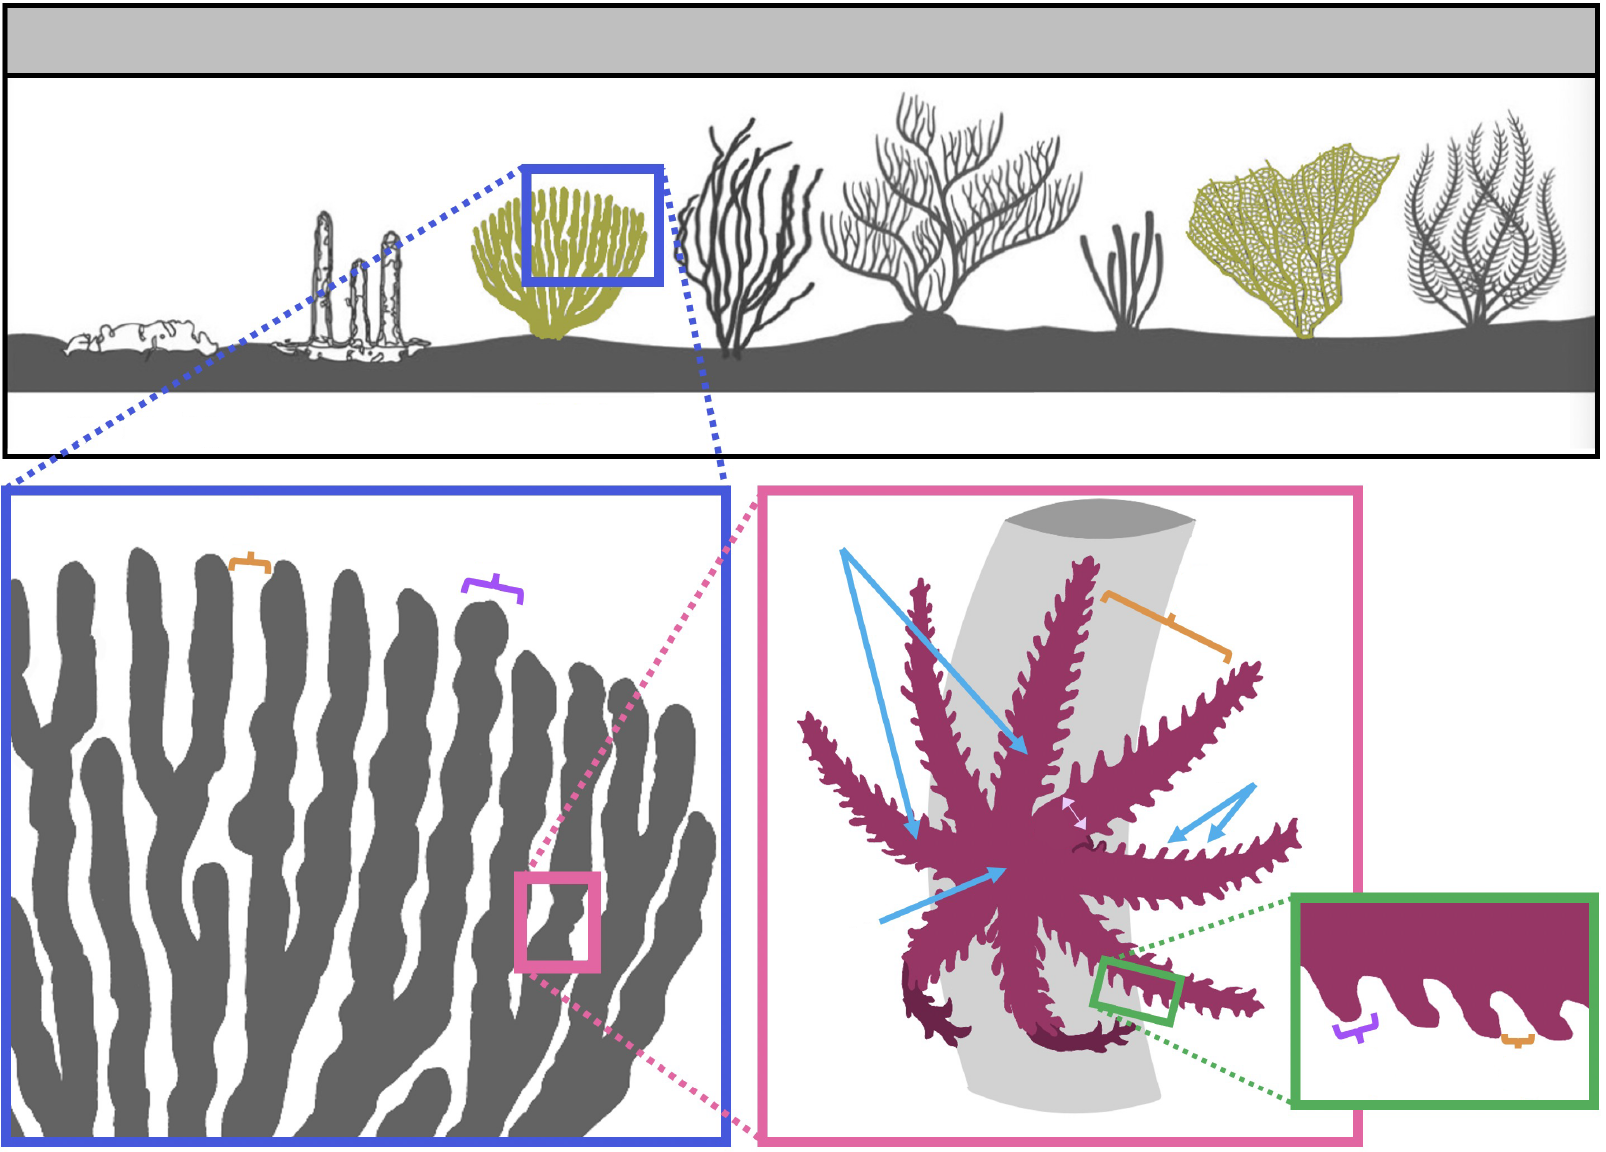
\includegraphics[width=\linewidth,height=0.48\textheight,keepaspectratio]{jeb2023-fig1-gorgonian-scales.png}
\source{Biological scales and gorgonian morphology: Hamlet et al. (2023), Fig.~1 (adapted from Kupfner Johnson \& Hallock, 2020), CC BY 4.0.}
\end{column}
\end{columns}
\vspace{4pt}
{\scriptsize A spatially varying \(\boldsymbol\sigma(\vect X)\) needs a Milstein-type scheme for strong order 1; the built-in Euler--Maruyama step is only order 0.5 in that case and does not support it directly.}
{\footnotesize\warn{One-way coupling.}
Agent motion does \emph{not} alter \(\vect u\); use a coupled solver when feedback matters.}
\end{frame}

% ----- 4. Workflow -----
\begin{frame}{The end-to-end workflow}
\centering
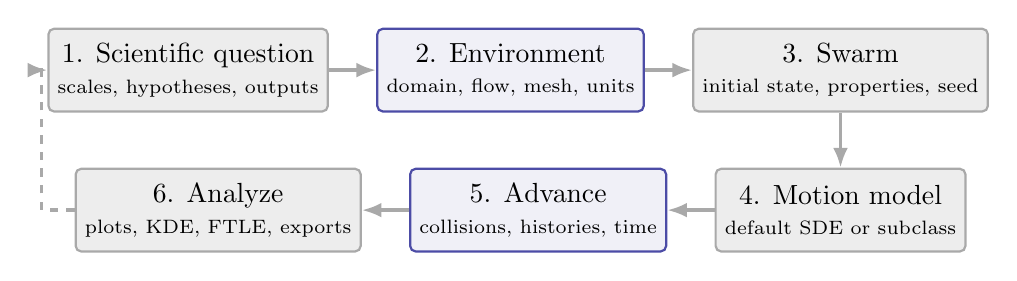
\begin{tikzpicture}[
  node distance=7mm and 6mm,
  box/.style={draw=DarkGray,thick,rounded corners=2pt,fill=LightGray!40,
              minimum width=3.0cm,minimum height=1.05cm,align=center},
  data/.style={draw=plankblue,thick,rounded corners=2pt,fill=NavyBlue!6,
               minimum width=3.0cm,minimum height=1.05cm,align=center},
  arr/.style={-{Latex[length=2.5mm]},very thick,plankgray}
]
\node[box] (question) {1. Scientific question\\[-1pt]\scriptsize scales, hypotheses, outputs};
\node[data,right=of question] (flow) {2. Environment\\[-1pt]\scriptsize domain, flow, mesh, units};
\node[box,right=of flow] (agents) {3. Swarm\\[-1pt]\scriptsize initial state, properties, seed};
\node[box,below=of agents] (behavior) {4. Motion model\\[-1pt]\scriptsize default SDE or subclass};
\node[data,left=of behavior] (advance) {5. Advance\\[-1pt]\scriptsize collisions, histories, time};
\node[box,left=of advance] (analyse) {6. Analyze\\[-1pt]\scriptsize plots, KDE, FTLE, exports};
\draw[arr] (question)--(flow);
\draw[arr] (flow)--(agents);
\draw[arr] (agents)--(behavior);
\draw[arr] (behavior)--(advance);
\draw[arr] (advance)--(analyse);
\draw[arr,dashed] (analyse.west) -- ++(-0.42,0) |- (question.west);
\end{tikzpicture}
\vspace{0.8em}
\begin{punchbox}
\centering
Treat plotting and diagnostics as part of the simulation loop: inspect early, then scale up.
\end{punchbox}
\source{Schematic: instructor's course notes.}
\end{frame}

% ----- 5. Install -----
\begin{frame}[fragile]{Install from the cloned repository}
Clone the official repository, then make an isolated environment inside it.
\begin{lstlisting}
git clone https://github.com/mountaindust/Planktos.git
cd Planktos
python -m venv .venv

# PowerShell
.\.venv\Scripts\Activate.ps1
# macOS/Linux: source .venv/bin/activate

python -m pip install --upgrade pip
python -m pip install -e .
python -c "import planktos; print(planktos.__version__)"
\end{lstlisting}
Expected version for this deck: \texttt{1.0.3}.

\begin{columns}[T,onlytextwidth]
\begin{column}{0.48\textwidth}
\begin{block}{Editable install}
\texttt{-e} points the environment at the clone, so a later \texttt{git pull} updates the import without reinstalling.
\end{block}
\end{column}
\begin{column}{0.48\textwidth}
\begin{block}{Smoke test}
Run \texttt{python examples/basic\_ex\_2d.py}; close each interactive plot to continue.
\end{block}
\end{column}
\end{columns}
\source{Adapted from the repository \texttt{README.md} Quickstart. Examples that read data files are run from \texttt{examples/}, as the documentation says.}
\end{frame}

% ----- 6. Dependencies -----
\begin{frame}[fragile]{Dependencies: what is installed, and what is optional}
\small
\begin{columns}[T,onlytextwidth]
\begin{column}{0.57\textwidth}
\begin{tabular}{@{}>{\raggedright\arraybackslash}p{0.30\linewidth}>{\raggedright\arraybackslash}p{0.62\linewidth}@{}}
\toprule
\textbf{Declared core} & \textbf{Role} \\
\midrule
Python \(\ge 3.8\) & runtime (development uses Python 3.12) \\
NumPy \(\ge 1.19\) & vectorized agent and field arrays \\
SciPy \(\ge 1.10.1\) & interpolation, KDE, ODE integration \\
Matplotlib \(\ge 3.0\) & plots and animations \\
pandas & per-agent properties \\
VTK/PyVista & \(\ge 9.2/\ge 0.44\); CFD/mesh I/O and VTK output \\
\bottomrule
\end{tabular}
\end{column}
\begin{column}{0.39\textwidth}
\begin{block}{Optional extras}
\begin{lstlisting}
python -m pip install -e ".[STL,netCDF,test]"
\end{lstlisting}
\begin{itemize}\itemsep2pt
  \item \texttt{numpy-stl}: STL input;
  \item \texttt{netCDF4}: NetCDF input;
  \item \texttt{pytest}: test suite.
\end{itemize}
\end{block}
\begin{alertblock}{VTK installation}
The project documentation highly recommends Miniforge (instead of Anaconda) and conda-forge for as much as possible, VTK and PyVista included.
\end{alertblock}
\end{column}
\end{columns}
\source{Versions and extras are from \texttt{setup.cfg} at commit \texttt{a1c2128}; the development Python and the Miniforge advice from \texttt{docs/quickstart.rst}.}
\end{frame}

% ----- 7. FFmpeg -----
\begin{frame}[fragile]{\NoCaseChange{FFmpeg} is needed only when saving animations}
\label{fr:ffmpeg}
\begin{columns}[T,onlytextwidth]
\begin{column}{0.52\textwidth}
\begin{lstlisting}
# Verify that the executable is on PATH
ffmpeg -version

# PowerShell can also locate it explicitly
Get-Command ffmpeg
\end{lstlisting}
\begin{block}{Without FFmpeg}
Simulations, static plots, and interactive animations still work. A filename passed to \texttt{plot\_all} triggers the external movie writer.
\end{block}
\end{column}
\begin{column}{0.44\textwidth}
\begin{alertblock}{If it is not found}
\begin{enumerate}\itemsep4pt
  \item install FFmpeg with the platform's package manager or official installer;
  \item add its executable directory to \texttt{PATH};
  \item restart the terminal or IDE;
  \item rerun \texttt{ffmpeg -version} in the same environment that runs Python.
\end{enumerate}
\end{alertblock}
\end{column}
\end{columns}
\begin{punchbox}
\centering
For long simulations, save every \(k\)-th state as a frame; rendering every time step is rarely useful.
\end{punchbox}
\end{frame}

% ----- 7b. Tests -----
\begin{frame}[fragile]{Running the tests}
\label{fr:tests}
\begin{lstlisting}
cd Planktos                      # the clone's base directory
python -m pip install pytest
pytest                           # the test suite
pytest --runslow                 # also the parallelization tests and the plotting smoke tests
\end{lstlisting}
\begin{itemize}\itemsep3pt
  \item The 2021 deck: ``All tests can be run by typing pytest into a terminal in the base directory.'' It is the same in 2026, and GitHub Actions run the suite and a spell check on pushes to the main branches and on pull requests (``with every push'', say the 1.0.1 notes), with Python 3.8 and 3.12.
  \item 1.0.2 grew the suite: the immersed-boundary collision code is covered to 99\,\%, with checks that do not depend on the geometry (no penetration, no amplification of motion, independence from position, axis orientation and units).
  \item Not run for this chapter: the package here was installed with \texttt{pip install git+\dots}, which brings no \texttt{tests} folder. The scripts of \texttt{examples/Planktos} (slide~\ref{fr:ourexamples}) ran instead.
\end{itemize}
\source{Planktos \texttt{README.md} (``Tests''; October 2026) and release notes v1.0.1, v1.0.2; ``Getting started with Planktos'' (Miller lab, 2021), slide 12.}
\end{frame}

% ----- 7c. Then and now -----
\begin{frame}{Installing, 2021 and 2026}
\label{fr:then}
\scriptsize
\begin{tabular}{@{}p{0.46\textwidth}p{0.48\textwidth}@{}}
\toprule
the lab's 2021 deck (``Getting started with Planktos'') & Planktos 1.0.3 (2026) \\
\midrule
Python 3.5+ & Python \(\ge 3.8\) (tested on 3.8 and 3.12) \\
download with git or GitHub Desktop, and pull often (``Christopher just fixed some bugs today'') & \texttt{git clone}, then \texttt{pip install .} or \texttt{pip install -e .}; pull often \\
NumPy, SciPy, Matplotlib 3.x, pandas & NumPy \(\ge 1.19\), SciPy \(\ge 1.10.1\) (``earlier versions have a broken interpn''), Matplotlib \(\ge 3.0\), pandas \\
FFmpeg from conda-forge (\texttt{conda install -c conda-forge ffmpeg}) & FFmpeg from anywhere, on the \texttt{PATH} (slide~\ref{fr:ffmpeg}) \\
VTK and PyVista from conda-forge, installed with mamba & VTK \(\ge 9.2\), PyVista \(\ge 0.44\); conda-forge and mamba still advised \\
numpy-stl for STL files & numpy-stl \(\ge 2.16.3\); netCDF4 \(\ge 1.5.7\) for NetCDF \\
pytest for the tests & the same, and \texttt{--runslow} (slide~\ref{fr:tests}) \\
IBAMR data: ``a Python 2.7 environment with numpy and VisIt installed (VisIt's Python API is written in Python 2.7)'' & VisIt's Python is 3 from VisIt 3.2 on (chapter 32): chapter 33's \texttt{resample\_export.py}, then \texttt{vtk\_for\_planktos.py} (slide~\ref{fr:ibamr}) \\
\bottomrule
\end{tabular}
\source{``Getting started with Planktos'' (Miller lab, 2021), slides 8--11; Planktos \texttt{README.md} (October 2026); chapter 32.}
\end{frame}

% ----- 7d. The 2021 examples -----
\begin{frame}{The 2021 examples, with today's names}
\label{fr:examples2021}
\scriptsize
\begin{tabular}{@{}p{0.25\textwidth}p{0.3\textwidth}p{0.39\textwidth}@{}}
\toprule
2021 & what it showed & in 1.0.3 (\texttt{examples/}) \\
\midrule
\texttt{example\_2d.py} & time-varying Brinkman flow across a porous layer & \texttt{basic\_ex\_2d.py} (Brinkman flow; the start of the tour) \\
\texttt{example\_3d.py}, \texttt{example\_3d\_flat.py} & the same in 3D; ``Same as previous but different dimensions in each direction'' & \texttt{basic\_ex\_3d.py} (a $20\times10\times4$ box) \\
\texttt{example\_IBAMR.py} & 3D flow around cylinders read from IBAMR & \texttt{ex\_IBAMR\_ibmesh.py}: IBAMR test data (dumps 3--5), a cylinder by convex hull, the domain tiled \\
\texttt{example\_IBAMR\_ibmesh.py} & agents around a cylinder in 3D, saved as a movie & the same file \\
\texttt{example\_IBAMR\_ind\_var.py} & a 2D Brinkman layer, agents that differ & \texttt{ex\_ind\_var.py} (\texttt{example\_ind\_var.py} in the 2021 repository): the covariance differs from agent to agent \\
an IB2d leaf (not on GitHub then) & IB2d flow past a leaf made from a vertex file & no leaf; \texttt{ex\_ib2d\_ibmesh.py} reads IB2d's flow around a cylinder (data from a link) \\
a COMSOL sea fan (not on GitHub then) & COMSOL flow through an STL sea fan & \texttt{ex\_sticky\_seafan\_3d.py}: a COMSOL cylinder tiled into an array, sticky (data from a link) \\
\bottomrule
\end{tabular}

\vspace{0.3mm}
\scriptsize New since 2021: \texttt{ex\_agent\_behavior.py}, \texttt{ex\_ode\_gen.py}, \texttt{ex\_poisson\_search.py}, \texttt{ex\_produce\_ftle\_2d.py}, \texttt{ex\_ib2d\_sticky.py}, \texttt{ex\_ib2d\_mvbnd\_sticky.py}, \texttt{ex\_vicsek\_model\_2d.py}, \texttt{ex\_vicsek\_model\_3d.py}. \texttt{old\_examples/} keeps \texttt{old\_example\_2d.py}, \texttt{old\_example\_3d.py}, \texttt{old\_ex\_pltcyl.py}.
\source{``Getting started with Planktos'' (Miller lab, 2021), slides 13--20; the repository's \texttt{examples/} folder and the files' docstrings (GitHub, 17 October 2026; 2021: commit \texttt{58cca0d}). The repository of June 2021 also had \texttt{example\_2d\_plankton\_agent.py}, \texttt{example\_ib2d\_ibmesh.py}, \texttt{plt\_cyl.py} and \texttt{basic\_brine\_shrimp/}, which the 2021 deck did not show.}
\end{frame}

% ----- 7e. The 2021 output (1/2) -----
\begin{frame}{The 2021 examples' output (1/2)}
\label{fr:out2021}
\centering
\begin{tabular}{@{}cc@{}}
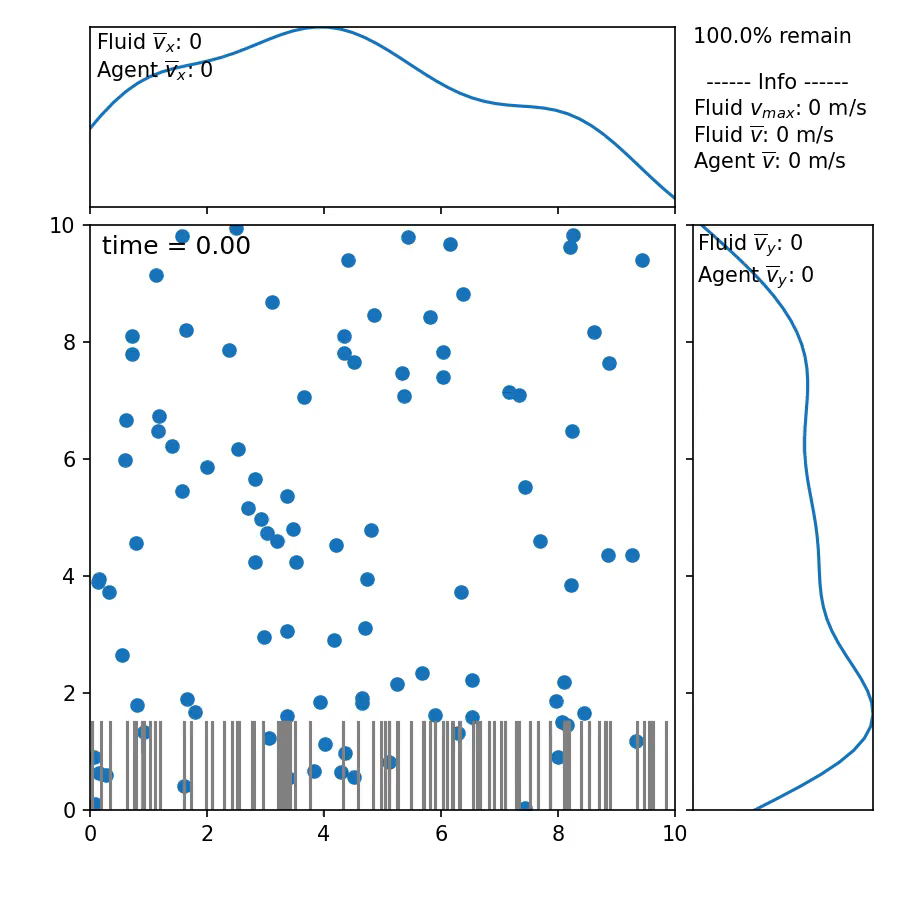
\includegraphics[height=0.33\textheight,keepaspectratio]{planktos-2021-example-2d.png} &
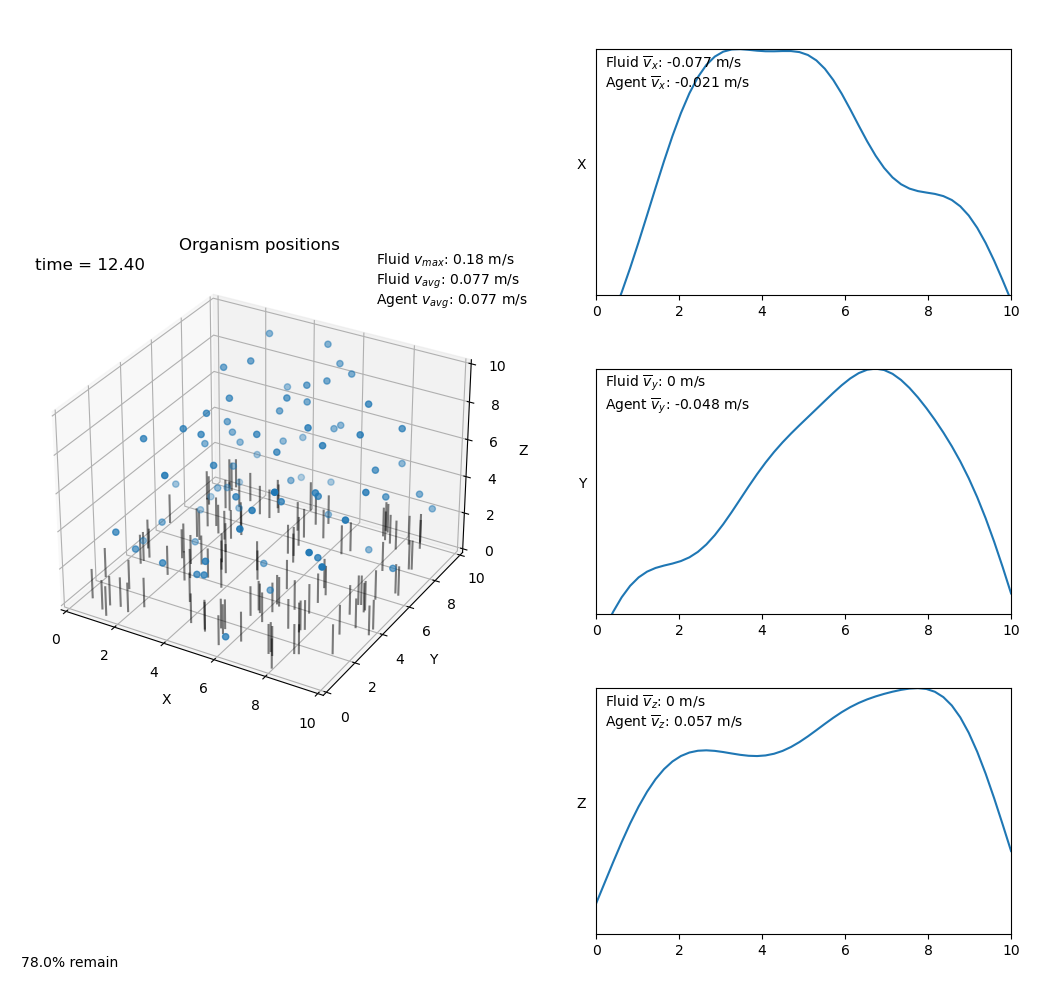
\includegraphics[height=0.33\textheight,keepaspectratio]{planktos-2021-example-3d.png} \\[-1pt]
\scriptsize \texttt{example\_2d.py}: Brinkman flow across a porous layer & \scriptsize \texttt{example\_3d.py}: the same in 3D \\[2pt]
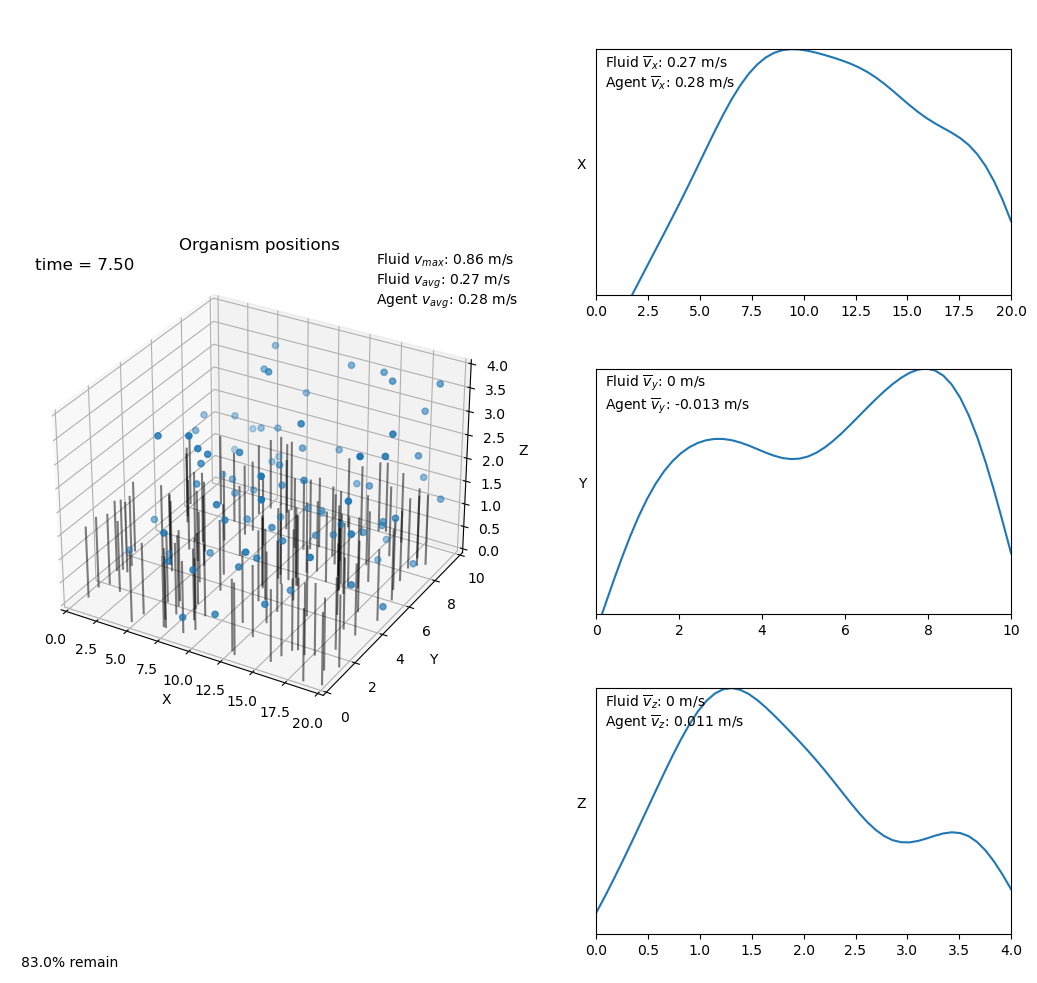
\includegraphics[height=0.33\textheight,keepaspectratio]{planktos-2021-example-3d-flat.png} &
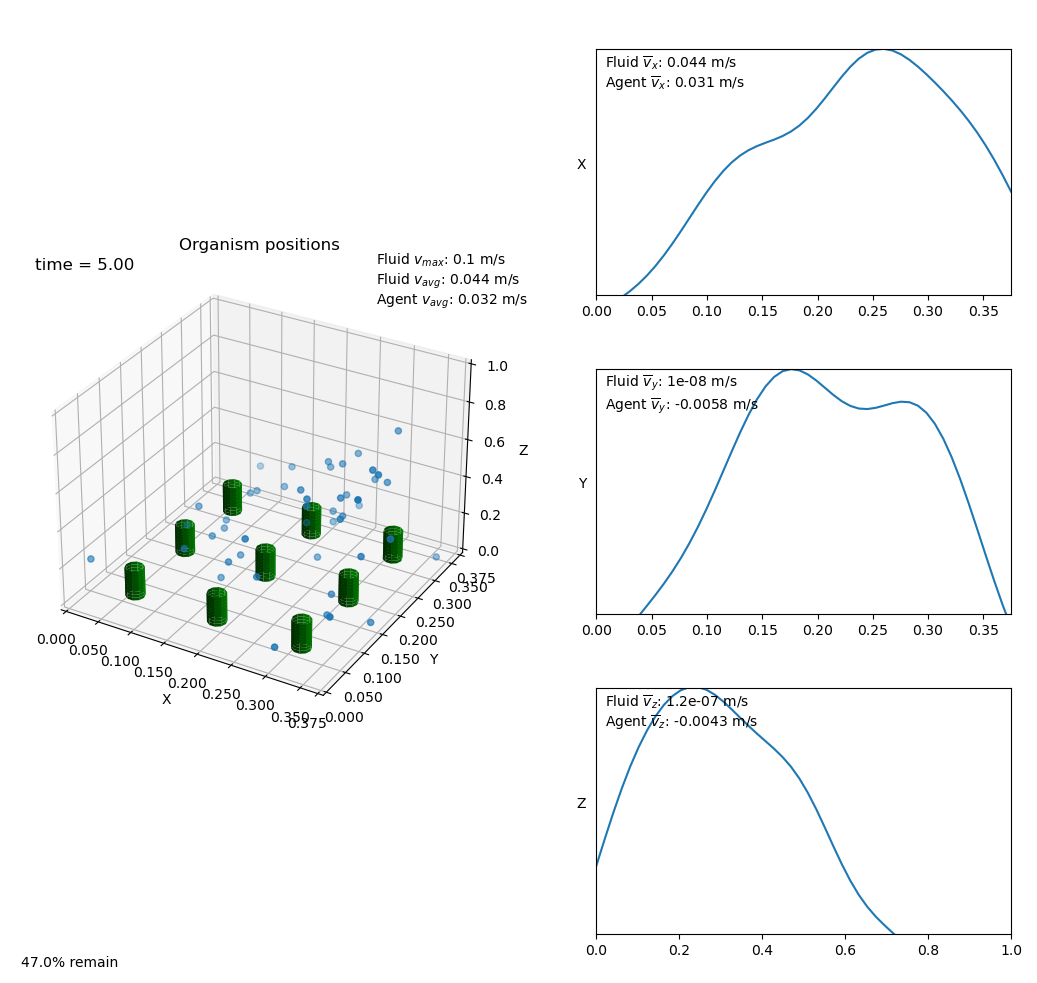
\includegraphics[height=0.33\textheight,keepaspectratio]{planktos-2021-example-ibamr.png} \\[-1pt]
\scriptsize \texttt{example\_3d\_flat.py}: different lengths in each direction & \scriptsize \texttt{example\_IBAMR.py}: IBAMR flow around cylinders \\
\end{tabular}
\source{Planktos output in ``Getting started with Planktos'' (Miller lab, 2021), slides 13--16.}
\end{frame}

% ----- 7f. The 2021 output (2/2) -----
\begin{frame}{The 2021 examples' output (2/2)}
\label{fr:out2021b}
\centering
\begin{tabular}{@{}cc@{}}
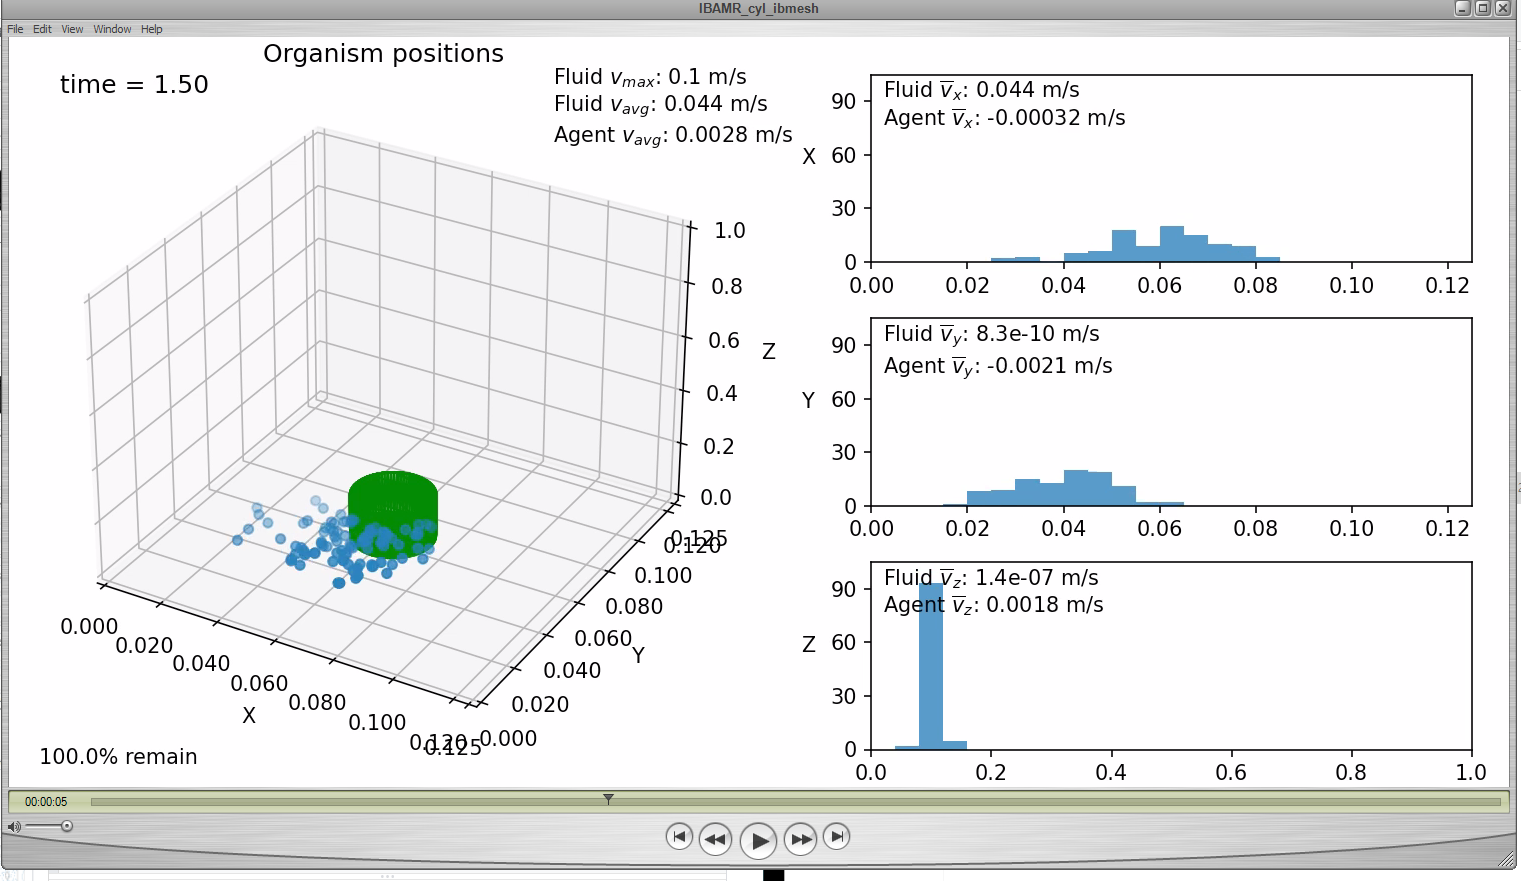
\includegraphics[height=0.33\textheight,keepaspectratio]{planktos-2021-example-ibamr-ibmesh.png} &
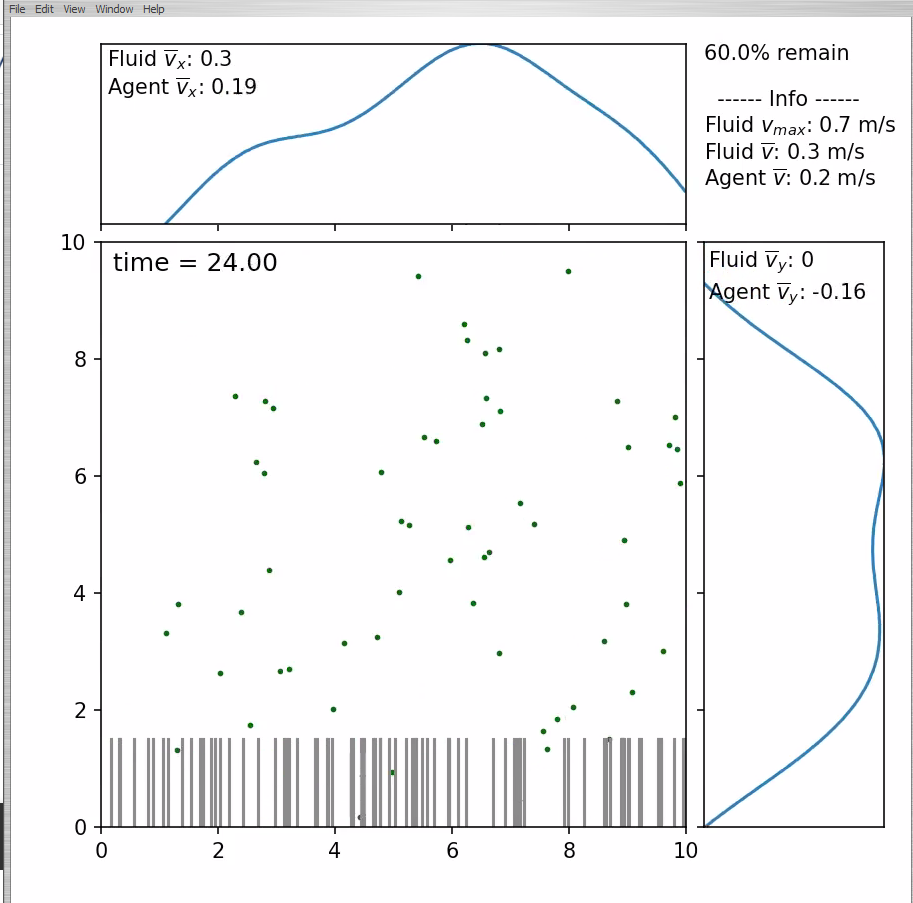
\includegraphics[height=0.33\textheight,keepaspectratio]{planktos-2021-example-ind-var.png} \\[-1pt]
\scriptsize \texttt{example\_IBAMR\_ibmesh.py}: a frame of its movie & \scriptsize \texttt{example\_IBAMR\_ind\_var.py}: agents that differ \\[2pt]
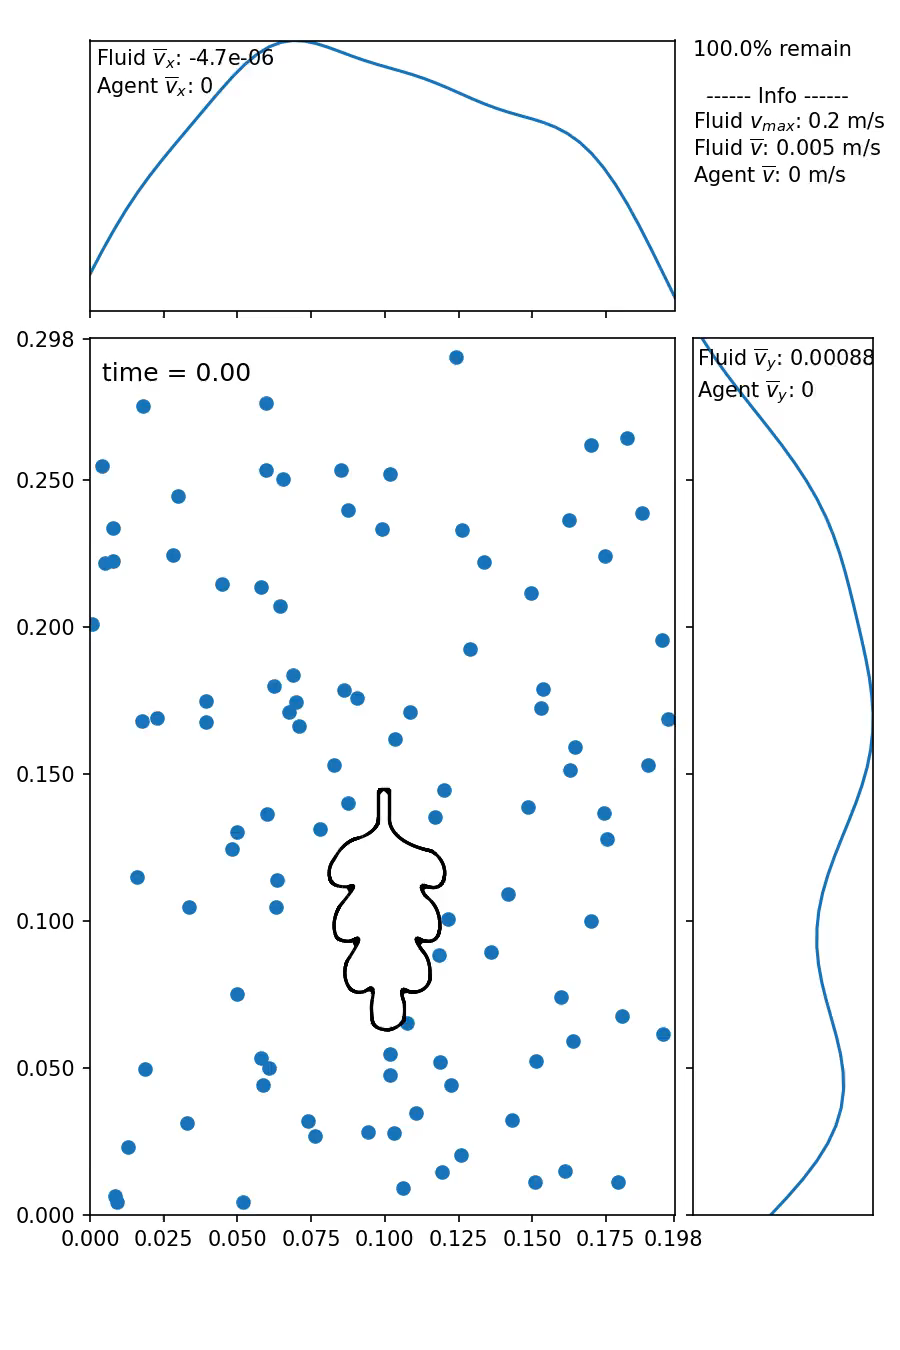
\includegraphics[height=0.33\textheight,keepaspectratio]{planktos-2021-ib2d-leaf.png} &
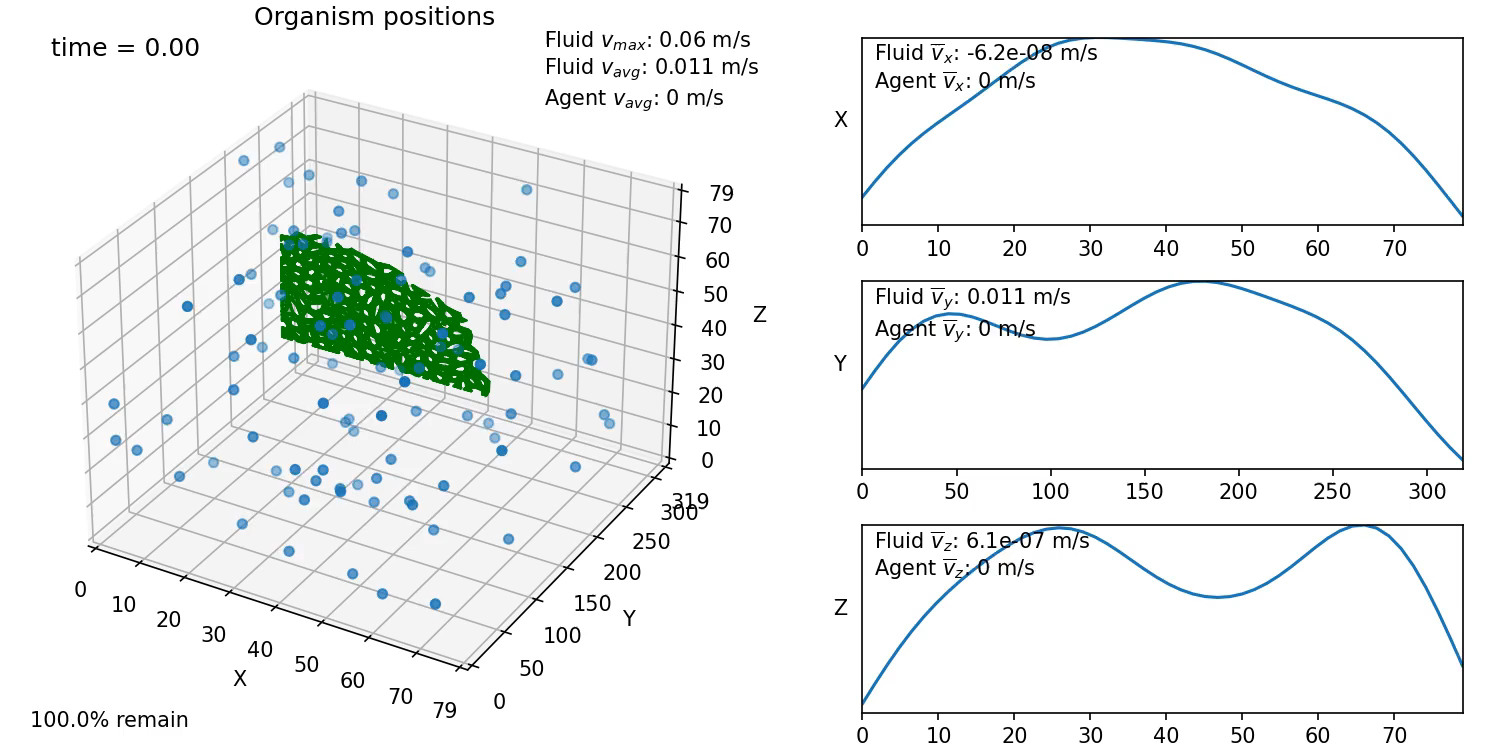
\includegraphics[height=0.33\textheight,keepaspectratio]{planktos-2021-comsol-seafan.png} \\[-1pt]
\scriptsize IB2d flow past a leaf (static mesh from a vertex file) & \scriptsize COMSOL flow through an STL sea fan \\
\end{tabular}
\source{Planktos output in ``Getting started with Planktos'' (Miller lab, 2021), slides 17--20.}
\end{frame}

% ----- 8. Object model -----
\begin{frame}{Two objects organize almost everything}
\centering
\begin{tikzpicture}[
  outer/.style={draw=DarkGray,thick,rounded corners=3pt,fill=LightGray!40,
                minimum width=13.4cm,minimum height=5.0cm},
  inner/.style={draw=plankteal,thick,rounded corners=2pt,fill=white,
                minimum width=3.4cm,minimum height=1.05cm,align=center}
]
\node[outer] (env) {};
\node[anchor=north west,font=\bfseries\large,text=BlackGray] at ([xshift=3mm,yshift=-3mm]env.north west)
  {\texttt{Environment}: the shared world};
\node[inner] at ([xshift=-4.25cm,yshift=0.85cm]env.center) {domain \(\vect L\)\\\scriptsize outer boundary conditions};
\node[inner] at ([xshift=0cm,yshift=0.85cm]env.center) {velocity field\\\scriptsize \texttt{flow}, grid, times};
\node[inner] at ([xshift=4.25cm,yshift=0.85cm]env.center) {immersed mesh\\\scriptsize static or time-dependent};
\node[inner,draw=plankgreen] at ([xshift=-3.0cm,yshift=-1.10cm]env.center) {\texttt{Swarm 1}\\\scriptsize positions, properties, histories};
\node[inner,draw=plankgreen] at ([xshift=1.05cm,yshift=-1.10cm]env.center) {\texttt{Swarm 2}\\\scriptsize independent behavior};
\node[inner,draw=plankorange] at ([xshift=4.75cm,yshift=-1.10cm]env.center) {clock\\\scriptsize \texttt{time}, \texttt{time\_history}};
\end{tikzpicture}
\vspace{0.55em}
\begin{itemize}\itemsep3pt
  \item A swarm is a vectorized group: agents are rows of NumPy arrays, not separate Python objects.
  \item All swarms in one environment sample the same flow and mesh.
\end{itemize}
\source{Schematic: instructor's course notes; object model from \texttt{planktos/\_environment.py} and \texttt{\_swarm.py}, commit \texttt{a1c2128}.}
\end{frame}

% ----- 9. First Environment -----
\begin{frame}[fragile]{Create the first environment}
\begin{columns}[T,onlytextwidth]
\begin{column}{0.56\textwidth}
\begin{lstlisting}
import planktos

env = planktos.Environment(
    Lx=20, Ly=5,
    x_bndry="zero",
    y_bndry=["noflux", "noflux"],
    rho=1000, mu=1.0,
    units="m")

print(env.L)       # [20, 5]
print(env.nu)      # mu/rho = 0.001
print(env.time)    # 0.0
\end{lstlisting}
\end{column}
\begin{column}{0.40\textwidth}
\begin{block}{Defaults worth knowing}
\begin{itemize}\itemsep4pt
  \item \(10\times10\) two-dimensional domain;
  \item zero velocity everywhere;
  \item \texttt{zero} boundaries in \(x,y\) (\texttt{noflux} in \(z\) when \texttt{Lz} is given);
  \item no swarms or immersed mesh;
  \item \texttt{time = 0.0}.
\end{itemize}
\end{block}
\begin{alertblock}{Units are metadata}
\texttt{units} does not rescale data automatically. Make the flow, mesh, agent parameters, gravity, and time convention consistent yourself.
\end{alertblock}
\end{column}
\end{columns}
\end{frame}

% ----- 10. Outer boundary conditions -----
\begin{frame}{Outer-domain boundary conditions}
\small
\begin{tabular}{@{}p{0.19\linewidth}p{0.48\linewidth}p{0.25\linewidth}@{}}
\toprule
\textbf{Setting} & \textbf{What happens to an agent crossing the box} & \textbf{Typical use} \\
\midrule
\texttt{zero} & The agent is masked and no longer updated or plotted. & open/outflow boundary \\
\texttt{noflux} & The proposed displacement through the wall is projected along it. & solid outer wall \\
\texttt{periodic} & The agent exits one side and re-enters on the opposite side. & repeating domain \\
\bottomrule
\end{tabular}

\vspace{0.6em}
\begin{columns}[T,onlytextwidth]
\begin{column}{0.53\textwidth}
Each axis accepts one string for both sides or a two-entry sequence:
\[
  \texttt{x\_bndry=["zero","noflux"]}.
\]
The order is low-side, high-side: left/right, bottom/top, and low/high \(z\).
\end{column}
\begin{column}{0.43\textwidth}
\begin{alertblock}{Do not conflate two layers}
These settings govern the rectangular domain. Immersed-mesh collisions are controlled separately by \texttt{ib\_condition} or \texttt{ib\_collisions}.
\end{alertblock}
\end{column}
\end{columns}
\end{frame}

% ----- 11. Analytical flow -----
\begin{frame}[fragile]{Generate a Brinkman-layer flow}
\label{fr:brinkman}
\begin{columns}[T,onlytextwidth]
\begin{column}{0.54\textwidth}
\begin{lstlisting}
env = planktos.Environment(
    Lx=20, Ly=5, rho=1000, mu=1000)

env.set_brinkman_flow(
    alpha=66, h_p=1.5,
    U=1, dpdx=1, res=101)

env.plot_flow()
\end{lstlisting}
\begin{itemize}\itemsep0pt
  \item \texttt{alpha}: inverse hydraulic-permeability parameter (\(\texttt{alpha}\to0\) is free flow; \texttt{alpha=0} itself stops with \texttt{ZeroDivisionError});
  \item \texttt{h\_p}: porous-layer height;
  \item \texttt{U}: velocity at the top of the domain;
  \item \texttt{dpdx}: pressure-gradient parameter;
  \item \texttt{res}: points across the resolved profile.
\end{itemize}
\end{column}
\begin{column}{0.42\textwidth}
\centering
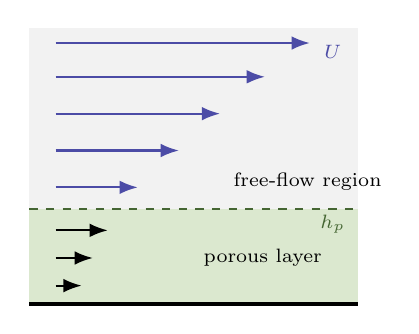
\begin{tikzpicture}[x=0.95cm,y=0.78cm,>=Latex]
  \fill[plankgreen!15] (0,0) rectangle (4.4,1.55);
  \fill[LightGray!30] (0,1.55) rectangle (4.4,4.5);
  \draw[very thick] (0,0)--(4.4,0);
  \draw[thick,dashed,plankgreen!70!black] (0,1.55)--(4.4,1.55);
  \draw[->,thick] (0.35,0.3)--(0.7,0.3);
  \draw[->,thick] (0.35,0.75)--(0.85,0.75);
  \draw[->,thick] (0.35,1.2)--(1.05,1.2);
  \draw[->,thick,plankblue] (0.35,1.9)--(1.45,1.9);
  \draw[->,thick,plankblue] (0.35,2.5)--(2.0,2.5);
  \draw[->,thick,plankblue] (0.35,3.1)--(2.55,3.1);
  \draw[->,thick,plankblue] (0.35,3.7)--(3.15,3.7);
  \draw[->,thick,plankblue] (0.35,4.25)--(3.75,4.25);
  \node[anchor=west] at (2.2,0.75){\scriptsize porous layer};
  \node[anchor=west] at (2.6,2.0){\scriptsize free-flow region};
  \node[anchor=east,plankgreen!70!black] at (4.35,1.3){\scriptsize \(h_p\)};
  \node[anchor=east,plankblue] at (4.3,4.1){\scriptsize \(U\)};
\end{tikzpicture}
\source{Code adapted from \texttt{examples/basic\_ex\_2d.py}. Schematic: instructor's course notes.}
\end{column}
\end{columns}
{\scriptsize The profile is the analytic, steady, fully developed solution of Brinkman's equation (Brinkman 1949; Strickland et al.\ 2017), with a Darcy drag \(-\alpha\mu\vect u\) in the porous layer per the docstring; the closed-form solution uses \(e^{-\alpha h_p}\), so check the units of \texttt{alpha} (inverse length there) before reusing values. \texttt{mu} and \texttt{rho} must be set, or the call raises.}
\end{frame}

% ----- 12. Flow representation -----
\begin{frame}[fragile]{Read the field representation before moving agents}
\small
\begin{columns}[T,onlytextwidth]
\begin{column}{0.54\textwidth}
\begin{lstlisting}
print(len(env.flow))
print([a.shape for a in env.flow])
print(env.flow_points)
print(env.flow_times)
print(env.L, env.units)
\end{lstlisting}
\begin{block}{Array convention}
\begin{itemize}\itemsep2pt
  \item static: \texttt{(nx, ny[, nz])};
  \item time-dependent: \texttt{(nt, nx, ny[, nz])};
  \item one array for each velocity component;
  \item \texttt{flow\_points[i]} indexes spatial axis \(i\).
\end{itemize}
\end{block}
\end{column}
\begin{column}{0.42\textwidth}
\begin{block}{Interpolation contract}
Planktos uses linear spatial interpolation on a rectilinear grid and cubic splines in time for time-dependent data.
\end{block}
\begin{alertblock}{Preflight checks}
{\footnotesize\begin{itemize}\itemsep0pt
  \item component shapes agree;
  \item coordinate arrays increase and match the axes;
  \item domain boundaries and mesh coordinates align;
  \item \texttt{flow\_times} spans the intended run;
  \item speeds and units are physically plausible.
\end{itemize}}
\end{alertblock}
\end{column}
\end{columns}
\end{frame}

% ----- 13. Hand-built field -----
\begin{frame}[fragile]{Supply a hand-built rectilinear velocity field}
\small
\begin{columns}[T,onlytextwidth]
\begin{column}{0.59\textwidth}
\begin{lstlisting}
import numpy as np
import planktos

x = np.linspace(0, 2, 81)
y = np.linspace(0, 1, 41)
X, Y = np.meshgrid(x, y, indexing="ij")

u = 4*Y*(1-Y)          # streamwise component
v = np.zeros_like(u)

env = planktos.Environment(
    Lx=x[-1], Ly=y[-1], flow=[u, v])
env.flow_points = (x, y)
env.plot_flow()
\end{lstlisting}
\end{column}
\begin{column}{0.37\textwidth}
\footnotesize
\begin{block}{Why \texttt{indexing="ij"}?}
Axis 0 is \(x\), axis 1 is \(y\). This matches the current Planktos storage convention and avoids a silent transpose.
\end{block}
\begin{block}{Time-dependent fields}
Stack snapshots on axis 0 and pass \texttt{flow\_times} to the constructor. The remaining axes stay \((x,y[,z])\).
\end{block}
\begin{alertblock}{Coordinates}
Set \texttt{flow\_points} explicitly when the coordinates are not the constructor's uniform grid.
\end{alertblock}
\end{column}
\end{columns}
\source{Convention cross-checked against current flow-generation and analysis tests.}
\end{frame}

% ----- 14. Add a Swarm -----
\begin{frame}[fragile]{Add a vectorized swarm}
\begin{columns}[T,onlytextwidth]
\begin{column}{0.57\textwidth}
\begin{lstlisting}
# Convenience method: automatically uses env
s = env.add_swarm(
    swarm_size=200,
    init="random", seed=2026,
    name="larvae", color="darkgreen")

# Equivalent explicit construction
s2 = planktos.Swarm(
    swarm_size=50, envir=env,
    init=(0.1, 0.5), seed=7)

print(s.N, s.positions.shape)
print(len(env.swarms))
\end{lstlisting}
\end{column}
\begin{column}{0.39\textwidth}
\begin{block}{State layout}
\begin{itemize}\itemsep4pt
  \item \texttt{positions}: masked \(N\times d\) array;
  \item \texttt{velocities}: \(N\times d\);
  \item \texttt{accelerations}: \(N\times d\);
  \item \texttt{props}: per-agent DataFrame;
  \item \texttt{shared\_props}: shared dictionary.
\end{itemize}
\end{block}
\begin{punchbox}
Vectorization is the design choice: write array operations over agents whenever possible.
\end{punchbox}
\end{column}
\end{columns}
\end{frame}

% ----- 15. Initial conditions -----
\begin{frame}[fragile]{Choose initial positions deliberately}
\label{fr:init}
\footnotesize
\begin{columns}[T,onlytextwidth]
\begin{column}{0.59\textwidth}
\begin{lstlisting}
# Uniform random over the domain
s_random = env.add_swarm(500, init="random", seed=1)

# One shared starting point
s_point = env.add_swarm(100, init=(0.15, 0.50), seed=2)

# Explicit N-by-d array
rng = np.random.default_rng(3)
xy = np.column_stack((
    rng.uniform(0.05, 0.15, 300),
    rng.uniform(0.20, 0.80, 300)))
s_patch = env.add_swarm(init=xy, seed=3)

# Grid, optionally excluding closed mesh interiors
s_grid = env.add_swarm(
    init="grid", grid_dim=(80, 40), testdir="x1")
\end{lstlisting}
\end{column}
\begin{column}{0.37\textwidth}
\begin{block}{Interpretation}
\begin{itemize}\itemsep2pt
  \item \texttt{random}: a uniform domain sample;
  \item point: a release cohort;
  \item \(N\times d\) array: measured or designed initial condition (its row count sets \(N\); \texttt{swarm\_size} is ignored);
  \item \texttt{grid}: transport-map or FTLE seed lattice.
\end{itemize}
\end{block}
\begin{alertblock}{Grid masking}
{\footnotesize\texttt{testdir} needs a loaded immersed mesh: without one the call above stops (``AttributeError: 'NoneType' object has no attribute 'reshape'''), so leave it out then. With a closed mesh, the chosen ray direction must give a robust inside/outside test.}
\end{alertblock}
\end{column}
\end{columns}
\end{frame}

% ----- 16. Properties and RNG -----
\begin{frame}[fragile]{Shared properties, individual variation, and seeds}
\begin{columns}[T,onlytextwidth]
\begin{column}{0.59\textwidth}
\begin{lstlisting}
import numpy as np

# Same for every agent
s.shared_props["mu"] = np.array([0.0, 0.0])
s.shared_props["cov"] = np.eye(2)*(0.01**2)
s.shared_props["diam"] = 1.0e-3

# One value per agent
rng = np.random.default_rng(2026)
s.props["swim_speed"] = rng.lognormal(
    mean=np.log(0.02), sigma=0.15, size=s.N)

# Uniform access: scalar/array as appropriate
speed = s.get_prop("swim_speed")
diam = s.get_prop("diam")
\end{lstlisting}
\end{column}
\begin{column}{0.37\textwidth}
\begin{block}{The two random streams}
\begin{itemize}\itemsep3pt
  \item \texttt{seed=} initializes \texttt{s.rndState}, used by built-in stochastic motion.
  \item A separate NumPy generator should seed any user-created initial conditions or properties.
\end{itemize}
\end{block}
\begin{alertblock}{Covariance units}
The default SDE uses step covariance \(\texttt{cov}\,dt\). Thus \texttt{cov} has units of length\(^2\)/time, not length\(^2\) per step.
\end{alertblock}
\end{column}
\end{columns}
\end{frame}

% ----- 17. Default SDE -----
\begin{frame}{The default model is Euler--Maruyama drift--diffusion}
\label{fr:sde}
For each active agent, the default \texttt{apply\_agent\_model} approximates
\[
  d\vect X
  = \left[\vect u(\vect X,t)+\vect\mu\right]dt
    + \boldsymbol\sigma\,d\vect W_t,
  \qquad
  \texttt{cov}=\boldsymbol\sigma\boldsymbol\sigma^{T}=2\boldsymbol D.
\]
One step is
\[
  \vect X^{n+1,*}=\vect X^n+
  \left[\vect u(\vect X^n,t^n)+\vect\mu\right]\Delta t
  +\mathcal N\!\left(\vect 0,\texttt{cov}\,\Delta t\right),
\]
followed by outer-boundary and immersed-mesh handling.

\begin{columns}[T,onlytextwidth]
\begin{column}{0.48\textwidth}
\begin{block}{Deterministic tracer}
For spatial dimension \(d\), set \texttt{mu = np.zeros(d)} and \texttt{cov = np.zeros((d,d))}; then motion is forward Euler using the local fluid velocity.
\end{block}
\end{column}
\begin{column}{0.48\textwidth}
\begin{alertblock}{Time-step audit}
Check both temporal convergence and collision resolution. A step can be statistically reasonable yet too large to resolve a narrow obstacle.
\end{alertblock}
\end{column}
\end{columns}
\source{Adapted from the \texttt{Swarm.apply\_agent\_model} and \texttt{motion.Euler\_brownian\_motion} docstrings (commit \texttt{a1c2128}); scheme: Kloeden \& Platen (1992), \S10.2. A \code{'D'} property (converted as \(\texttt{cov}=2D\)) is read only when there is no \code{'cov'}, and every Swarm starts with \code{cov} = the identity unless given one: delete it first (\code{del s.shared\_props['cov']}).}
\end{frame}

% ----- 18. Advance and history -----
\begin{frame}[fragile]{Advance the swarm and read its histories}
\small
\begin{columns}[T,onlytextwidth]
\begin{column}{0.58\textwidth}
\begin{lstlisting}
import numpy as np

dt = 0.1
for _ in range(round(24.0/dt)):
    s.move(dt, silent=True)

print(env.time)
print(len(env.time_history))
print(len(s.full_pos_history))

# Current diagnostics
mask = np.ma.getmaskarray(s.positions)
active = ~np.all(mask, axis=1)
print(active.sum(), "agents remain active")
print(s.velocities.mean(axis=0))
\end{lstlisting}
\end{column}
\begin{column}{0.38\textwidth}
\begin{block}{What \texttt{move} manages}
\begin{enumerate}\itemsep2pt
  \item calls \texttt{apply\_agent\_model(dt)};
  \item stores prior position/velocity/property state;
  \item estimates velocity and acceleration;
  \item applies boundaries and mesh collisions;
  \item calls \texttt{after\_move(dt)};
  \item advances environment time.
\end{enumerate}
\end{block}
{\scriptsize\hi{History note:} \texttt{full\_pos\_history} and \texttt{full\_vel\_history} return stored history plus the current state without mutating it.}
\end{column}
\end{columns}
\end{frame}

% ----- 19. Multiple swarms -----
\begin{frame}[fragile]{Move multiple swarms on one shared clock}
\begin{columns}[T,onlytextwidth]
\begin{column}{0.56\textwidth}
\begin{lstlisting}
tracers = env.add_swarm(
    500, seed=10, name="tracers", color="navy")
swimmers = env.add_swarm(
    500, seed=11, name="swimmers", color="orange")
swimmers.shared_props["mu"] = np.array([0.02, 0.0])

for _ in range(400):
    env.move_swarms(
        dt=0.05,
        ib_collisions="sliding",
        silent=True)
\end{lstlisting}
{\small\hi{Default differs:} \texttt{move\_swarms} uses \texttt{ib\_collisions="sliding"} unless told otherwise, overriding each swarm's \texttt{ib\_condition}; pass \texttt{ib\_collisions="default"} to honor each swarm's own setting.\par}
\end{column}
\begin{column}{0.40\textwidth}
\centering
\begin{tikzpicture}[>=Latex]
  \draw[thick,draw=DarkGray,rounded corners,fill=LightGray!40] (0,0) rectangle (4.8,4.0);
  \node[font=\bfseries,text=BlackGray] at (2.4,3.63){one \texttt{Environment}};
  \draw[->,very thick,plankorange] (0.6,3.0)--(4.2,3.0) node[midway,above]{\scriptsize shared clock};
  \node[draw=plankblue,fill=white,rounded corners] at (1.45,2.05){\scriptsize tracer swarm};
  \node[draw=plankorange,fill=white,rounded corners] at (3.45,2.05){\scriptsize swimmer swarm};
  \draw[->,plankblue,thick] (1.45,1.75)--(1.45,0.75);
  \draw[->,plankorange,thick] (3.45,1.75)--(3.45,0.75);
  \node[align=center] at (2.4,0.40){\scriptsize histories align at every\\[-1pt]\scriptsize environment time};
\end{tikzpicture}
\begin{alertblock}{Avoid double time advancement}
Do not call \texttt{s1.move(dt)} and then \texttt{s2.move(dt)} when both should occupy the same time step. Use \texttt{env.move\_swarms}.
\end{alertblock}
\source{Schematic: instructor's course notes.}
\end{column}
\end{columns}
\end{frame}

% ----- 20. Static plotting -----
\begin{frame}[fragile]{Make an early diagnostic plot}
\label{fr:plot}
\begin{columns}[T,onlytextwidth]
\begin{column}{0.52\textwidth}
\begin{lstlisting}
# Current state with velocity arrows
s.plot(
    fluid="quiver",
    dist="density",
    circ_rad=0.08,
    plot_heading=False)

# Closest stored state to t=8.0
s.plot(
    t=8.0,
    filename="snapshot.png",
    fluid="vort",
    save_kwargs={"dpi": 200})
\end{lstlisting}
\begin{block}{2D fluid overlays}
\texttt{fluid="quiver"} shows velocity vectors; \texttt{fluid="vort"} shows scalar vorticity. These overlays are 2D-only.
\end{block}
\end{column}
\begin{column}{0.45\textwidth}
\centering
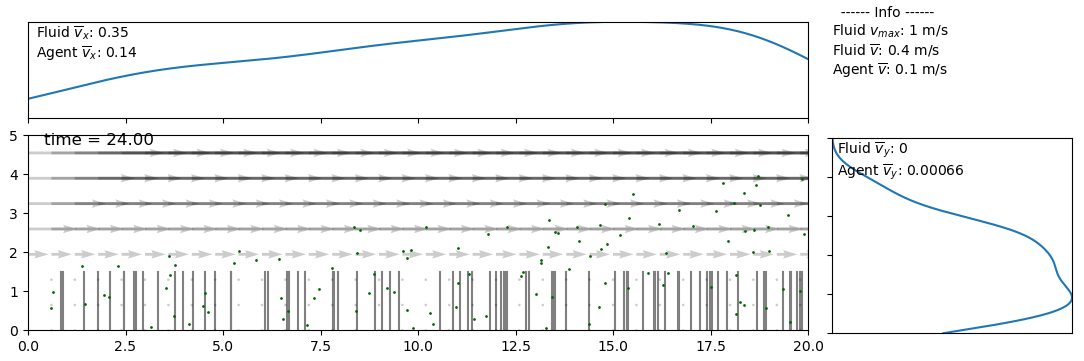
\includegraphics[width=\linewidth,height=0.63\textheight,keepaspectratio]{planktos-brinkman-agents.png}
\source{The first call above, run: \texttt{examples/Planktos/brinkman\_first.py} runs most of this chapter's first-run fragments, in order (Planktos 1.0.3): 200 agents in the Brinkman flow at \(t=24\) s, 110 of them still in the box (the default \texttt{zero} boundaries remove the rest). The documentation's own render of this example (\texttt{docs/\_static/basic\_ex\_2d\_agents.png}, GPLv3) is on the title slide.}
\end{column}
\end{columns}
\end{frame}

% ----- 21. KDE -----
\begin{frame}[fragile]{KDE turns particles into a distribution diagnostic}
\label{fr:kde}
\small
\begin{columns}[T,onlytextwidth]
\begin{column}{0.49\textwidth}
\begin{lstlisting}
# Gaussian KDE with Scott's factor
s.plot(dist="density", fluid="vort")

# Covariance-based width
s.plot(dist="cov", fluid="vort")

# User bandwidth factor or a histogram
s.plot(dist=0.35)
s.plot(dist="hist")
\end{lstlisting}
\begin{itemize}\itemsep0pt
  \item Compare concentration shape, tails, and obstacle wakes.
  \item Report the bandwidth rule with any quantitative comparison.
  \item Check sensitivity to sample size and boundary truncation.
  \item A KDE is a smoothed estimator, not a separately solved concentration field.
\end{itemize}
\end{column}
\begin{column}{0.48\textwidth}
\centering
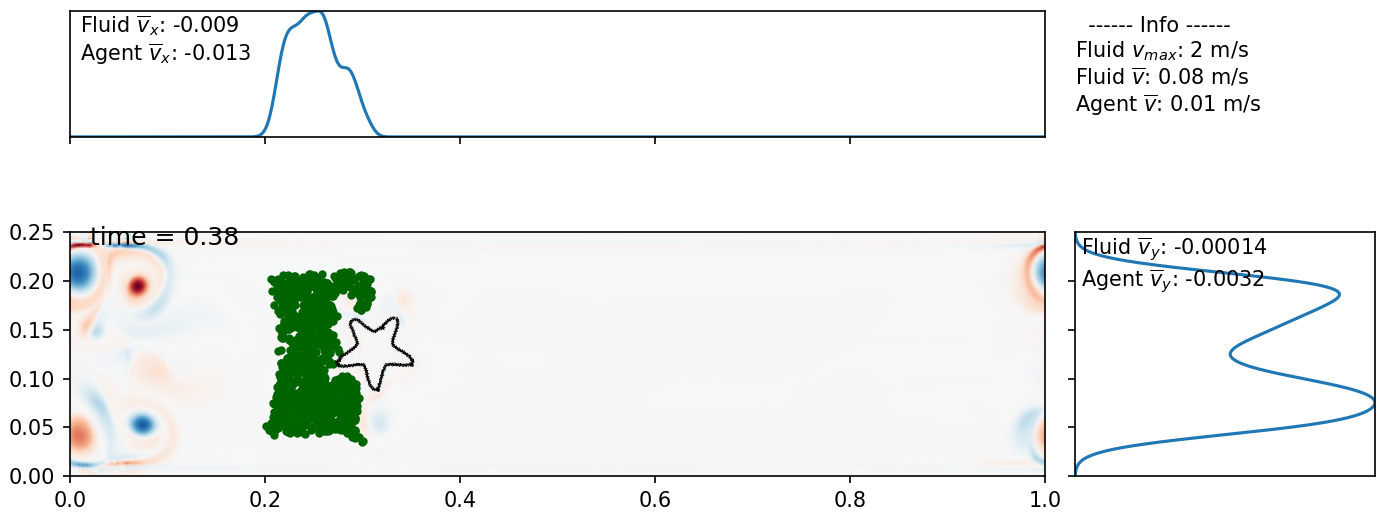
\includegraphics[width=\linewidth,height=0.51\textheight,keepaspectratio]{planktos-starfish-kde.png}
\source{\texttt{dist="density"} with \texttt{fluid="vort"} on this series' flow: 1000 agents released just upstream of chapter 4f's starfish, at \(t=0.38\) s; the KDE of \(y\) has a peak on each side of the starfish (\texttt{examples/Planktos/starfish\_kde.py}). Strickland et al.\ (2022), Fig.~4, shows the same kind of plot for an IB2d cylinder flow (not reproduced: the article is not openly licensed).}
\end{column}
\end{columns}
\end{frame}

% ----- 22. Animation and export -----
\begin{frame}[fragile]{Animate selectively; export analysis-ready data}
\label{fr:animate}
\small
\begin{columns}[T,onlytextwidth]
\begin{column}{0.60\textwidth}
\begin{lstlisting}
# Use every fifth stored state
frames = range(0, len(s.full_pos_history), 5)
s.plot_all(
    movie_filename="trial_01.mp4",
    frames=frames, fps=10,
    fluid="quiver", plot_heading=False)

# Data products
s.save_data("results", "trial_01")
s.save_pos_to_csv("results/trial_01_positions.csv")
s.save_pos_to_vtk("results", "trial_01")
\end{lstlisting}
{\footnotesize\hi{What \texttt{save\_data} writes:} CSV files for the position history (with mask and time stamps) and for the current velocities and accelerations; \texttt{props} to JSON; \texttt{shared\_props} to .npz. \texttt{props\_history} is not saved. \texttt{save\_pos\_to\_vtk} writes one PolyData file per stored time. \hi{Why \texttt{quiver}:} on a static flow such as this Brinkman layer, \texttt{plot\_all(fluid="vort")} stops in 1.0.3 (``ValueError: not enough values to unpack (expected 2, got 1)'') before a frame is drawn (slide~\ref{fr:issues2}).\par}
\end{column}
\begin{column}{0.36\textwidth}
\begin{block}{Choose the product by use}
\begin{itemize}\itemsep1pt
  \item \texttt{save\_data}: position history plus current kinematics and properties (file formats at left);
  \item CSV: portable position history;
  \item VTK: ParaView/VisIt workflow;
  \item MP4: communication, not raw data.
\end{itemize}
\end{block}
\begin{alertblock}{Cost control}
{\footnotesize Use \texttt{frames} for temporal subsampling and \texttt{downsamp} for display-only agent subsampling. Statistics still use the full population.}
\end{alertblock}
\end{column}
\end{columns}
\vspace{-2pt}
\source{Calls match current \texttt{Swarm.plot\_all} and save-method signatures.}
\end{frame}

% ----- 23. Subclass contract -----
\begin{frame}[fragile]{Custom behavior: override one hook, not the harness}
\begin{columns}[T,onlytextwidth]
\begin{column}{0.53\textwidth}
\begin{lstlisting}
class MySwarm(planktos.Swarm):
    def apply_agent_model(self, dt):
        # Compute proposed N-by-d positions.
        new_positions = ...
        return new_positions
\end{lstlisting}
\begin{block}{Contract}
\begin{itemize}\itemsep3pt
  \item keep the signature \texttt{(self, dt)};
  \item return an \(N\times d\) array;
  \item do not assign \texttt{positions}, \texttt{velocities}, or \texttt{accelerations};
  \item let \texttt{move} record history and apply collisions.
\end{itemize}
\end{block}
\end{column}
\begin{column}{0.43\textwidth}
\begin{alertblock}{Current versus historical API}
The 2022 paper describes a historical override named \texttt{get\_positions}. The current v1.0.3 repository and examples use \texttt{apply\_agent\_model(self, dt)}.
\end{alertblock}
\begin{punchbox}
\raggedright
Use \texttt{after\_move(dt)} for state changes based on the accepted, collision-corrected endpoint.
\end{punchbox}
\end{column}
\end{columns}
\source{Current contract: \texttt{planktos/\_swarm.py} and \texttt{examples/ex\_agent\_behavior.py}.}
\end{frame}

% ----- 24. Custom deterministic behavior -----
\begin{frame}[fragile]{Example: fluid advection plus directed swimming}
\begin{columns}[T,onlytextwidth]
\begin{column}{0.61\textwidth}
\begin{lstlisting}
import numpy as np
import planktos

class TargetSwarm(planktos.Swarm):
    def apply_agent_model(self, dt):
        target = np.array([1.8, 0.5])
        direction = target - self.positions
        norm = np.linalg.norm(direction, axis=1)[:, None]
        direction = direction/np.maximum(norm, 1.0e-12)

        speed = self.get_prop("swim_speed")[:, None]
        velocity = self.get_fluid_drift() + speed*direction
        return self.positions + velocity*dt
\end{lstlisting}
\end{column}
\begin{column}{0.35\textwidth}
\begin{block}{Useful field queries}
{\scriptsize
\begin{itemize}\itemsep2pt
  \item \texttt{get\_fluid\_drift()};
  \item \texttt{get\_dudt()};
  \item \texttt{get\_fluid\_mag\_gradient()};
  \item \texttt{get\_DuDt()}.
\end{itemize}}
\end{block}
\begin{alertblock}{Numerical hygiene}
Guard normalizations, preserve masks, and call expensive interpolants once per time step rather than once per agent.
\end{alertblock}
\end{column}
\end{columns}
\source{Pattern adapted from \texttt{examples/ex\_agent\_behavior.py}.}
\end{frame}

% ----- 25. ODE motion -----
\begin{frame}[fragile]{Deterministic ODE motion with the \NoCaseChange{RK45} wrapper}
\begin{columns}[T,onlytextwidth]
\begin{column}{0.60\textwidth}
\begin{lstlisting}[basicstyle=\densecode]
import planktos
from planktos import motion

class AccurateTracer(planktos.Swarm):
    def apply_agent_model(self, dt):
        ode = motion.tracer_particles(
            self, incl_dvdt=False)
        t0 = self.envir.time
        # positions is a masked array; strip masked
        # (exited) rows before RK45, as calculate_FTLE does
        return motion.RK45(
            ode, t0, self.positions.copy(), t0 + dt,
            rtol=1.0e-6, atol=1.0e-9)
\end{lstlisting}
{\footnotesize\hi{About the comment:} for brevity the listing passes the whole masked array. SciPy drops the mask, so exited rows are integrated from stale coordinates. Strip them as \texttt{calculate\_FTLE} does, \texttt{y = pos[\textasciitilde mask[:,0]]}, and scatter the result back. (\texttt{incl\_dvdt=False} makes the tracer ODE act on \(N\times d\) positions only.)\par}
\end{column}
\begin{column}{0.36\textwidth}
\begin{block}{Current solver contract}
\texttt{motion.RK45} wraps SciPy \texttt{solve\_ivp}; the right-hand side has signature \texttt{fun(t, x)} and returns the same 2D shape as \texttt{x}.
\end{block}
\begin{alertblock}{Two time scales}
The internal ODE solver adapts substeps, but Planktos applies boundary and mesh collision handling only after the outer \texttt{move(dt)} proposal.
\end{alertblock}
\end{column}
\end{columns}
\end{frame}

% ----- 26. SDE with ODE drift -----
\begin{frame}[fragile]{Combine an ODE drift with stochastic motion}
\begin{columns}[T,onlytextwidth]
\begin{column}{0.60\textwidth}
\begin{lstlisting}
import numpy as np
import planktos
from planktos import motion

def social_bias(pos):
    return 0.1*(pos.mean(axis=0) - pos)

def behavior_ode(swarm):
    def rhs(t, x):
        N = x.shape[0]//2
        vel = swarm.get_fluid_drift(t, x[:N])
        vel += social_bias(x[:N])
        return np.concatenate((
            vel, np.zeros((N, x.shape[1]))))
    return rhs

class SocialSwarm(planktos.Swarm):
    def apply_agent_model(self, dt):
        return motion.Euler_brownian_motion(
            self, dt, ode=behavior_ode(self))
\end{lstlisting}
\end{column}
\begin{column}{0.36\textwidth}
\footnotesize
\begin{block}{State convention}
An ODE passed to \texttt{Euler\_brownian\_motion} receives \(2N\times d\): positions followed by velocities. It returns their time derivatives in the same layout.
\end{block}
\begin{alertblock}{Fluid drift is explicit}
When an \texttt{ode} is supplied, include fluid interaction in that ODE if it is part of the model; it is not added automatically there.
\end{alertblock}
{\scriptsize The swarm's \texttt{mu} property is still added to the ODE's velocity rows (zero by default), and the step is the Taylor update \(\Delta\vect x=\vect v\,\Delta t+\tfrac12\vect a\,\Delta t^2\) plus the \texttt{cov} noise.\par}
\end{column}
\end{columns}
\source{Adapted from \texttt{examples/ex\_ode\_gen.py}.}
\end{frame}

% ----- 27. Inertial particles (1/2) -----
\begin{frame}[fragile]{Built-in inertial-particle dynamics (1/2)}
\label{fr:inertial}
\footnotesize
{\scriptsize\warn{Set \(\rho\), \(\mu\), \(\nu\) in the constructor:} the constructor computes the third value correctly, but in v1.0.3 the \texttt{nu} and \texttt{rho} property setters compute \(\mu=\nu/\rho\) instead of \(\mu=\nu\rho\) when \(\mu\) is unset (an upstream bug, still present on \texttt{master} as of October 2026; not yet filed as a GitHub issue).}
\begin{columns}[T,onlytextwidth]
\begin{column}{0.45\textwidth}
\begin{lstlisting}[basicstyle=\ttfamily\scriptsize]
import numpy as np
import planktos
from planktos import motion

zero = np.zeros((3, 3))
env = planktos.Environment(
    Lx=1, Ly=1, rho=1000, nu=1e-6,
    char_L=0.01, U=0.1,
    flow=[zero, zero.copy()])
\end{lstlisting}
{\scriptsize The listing continues on the next slide with the Swarm subclass. Here \(\mathrm{Re}=U\,\texttt{char\_L}/\nu=0.1\cdot0.01/10^{-6}=1000\), and the constructor sets \(\mu=\nu\rho=10^{-3}\).\par\smallskip
More on the setters: once all three are set, a setter only warns and leaves the other two unchanged. The bug is still on \texttt{master} (last commit 2026-09-16); no public GitHub issue for it was found as of 2026-10-17.}
\end{column}
\begin{column}{0.52\textwidth}
\footnotesize
\begin{block}{Required environment data}
\footnotesize A velocity field (explicit zeros are valid), \texttt{char\_L}, \texttt{U}, \texttt{nu}, and gravity; fluid density unless \texttt{R} is supplied.
\end{block}
\begin{block}{Required particle data}
\footnotesize Density ratio \texttt{R} (or particle \texttt{rho}) and diameter \texttt{diam}.
\end{block}
\begin{alertblock}{Model regime}
\footnotesize The implementation is the linearized Maxey--Riley form documented for \(R/\mathrm{St}\gg1\); verify that approximation for the particles and flow under study. Here, the displayed parameters (with \texttt{R} and \texttt{diam} from slide 2/2) give \(R/\mathrm{St}\approx120\).
\end{alertblock}
\end{column}
\end{columns}
\source{Setter behavior: \texttt{Environment.rho/mu/nu} in \texttt{planktos/\_environment.py}, commit \texttt{a1c2128}.}
\end{frame}

% ----- 27b. Inertial particles (2/2) -----
\begin{frame}[fragile]{Built-in inertial-particle dynamics (2/2)}
\begin{columns}[T,onlytextwidth]
\begin{column}{0.61\textwidth}
\begin{lstlisting}[basicstyle=\ttfamily\scriptsize]
class InertialSwarm(planktos.Swarm):
    def apply_agent_model(self, dt):
        ode = motion.inertial_particles(self)
        # positions is a masked array; strip masked
        # (exited) rows before RK45, as calculate_FTLE does
        # NB: move() overwrites velocities with
        # (x_new-x_old)/dt; persist velocity in props
        # for a true second-order model
        state = np.ma.concatenate(
            (self.positions, self.velocities))
        out = motion.RK45(
            ode, self.envir.time, state,
            self.envir.time + dt)
        return out[:self.N]

s = InertialSwarm(envir=env, seed=4)
s.shared_props.update({"R": 2/3, "diam": 1e-4})
\end{lstlisting}
{\scriptsize\hi{Units:} Planktos applies the dimensionless equation at right to the data's metres and seconds, so the slip here decays at \(R/\mathrm{St}=120\) s\(^{-1}\) (measured), while the physical rate is \((R/\mathrm{St})\,U/\texttt{char\_L}=3\nu/a^2=1200\) s\(^{-1}\): use units with \(U=\texttt{char\_L}\), or rescale.\par}
\end{column}
\begin{column}{0.36\textwidth}
\small
\begin{block}{The ODE being integrated}
\scriptsize With state \((\vect x,\vect v)\) stacked as \(2N\times d\),
\[
  \dot{\vect v}=\tfrac{3R}{2}\tfrac{D\vect u}{Dt}-\tfrac{R}{\mathrm{St}}(\vect v-\vect u)+\big(1-\tfrac{3R}{2}\big)\vect g,
\]
\(R=\dfrac{2\rho_f}{\rho_f+2\rho_p}\), \(\mathrm{St}=\tfrac29\big(\tfrac{a}{L}\big)^2\mathrm{Re}\), \(a=\texttt{diam}/2\).
\end{block}
{\scriptsize Check: \(\mathrm{St}=\tfrac29(5\times10^{-3})^2\cdot1000\approx5.6\times10^{-3}\), so \(R/\mathrm{St}\approx0.667/0.0056\approx120\). \(R=2/3\) is neutrally buoyant, so the gravity term vanishes.}
\end{column}
\end{columns}
\source{Model: \texttt{motion.inertial\_particles} docstring, after Maxey \& Riley (1983) and Haller \& Sapsis (2008).}
\end{frame}

% ----- 28. Collision modes -----
\begin{frame}{Immersed-mesh collision modes}
\label{fr:collide}
\small
\begin{columns}[T,onlytextwidth]
\begin{column}{0.48\textwidth}
\scriptsize
\begin{tabular}{@{}p{0.24\linewidth}p{0.67\linewidth}@{}}
\toprule
\textbf{Mode} & \textbf{Proposed step after a mesh hit} \\
\midrule
\texttt{sliding} & Project motion along the boundary, recursively using remaining displacement. \\
\texttt{sticky} & Stop at the first point of intersection for that time step. \\
\texttt{None} & Ignore immersed meshes. \\
\code{'default'} & Use the Swarm's \texttt{ib\_condition} (default \code{'sliding'}). \\
\bottomrule
\end{tabular}
\vspace{0.5em}
Set a swarm default with \texttt{ib\_condition}; override per step with
\[
 \texttt{s.move(dt, ib\_collisions="sticky")}.
\]
\texttt{s.ib\_collision\_idx} is a per-agent array of the last-step element index hit, \(-1\) if none: precisely, the element of the \emph{first} intersection during the most recent step (a sliding agent may go on to touch others). It is reset every step for agents still in the domain, so a captured agent held in place reads \(-1\) on later steps; keep capture in \texttt{props}.
\end{column}
\begin{column}{0.49\textwidth}
\centering
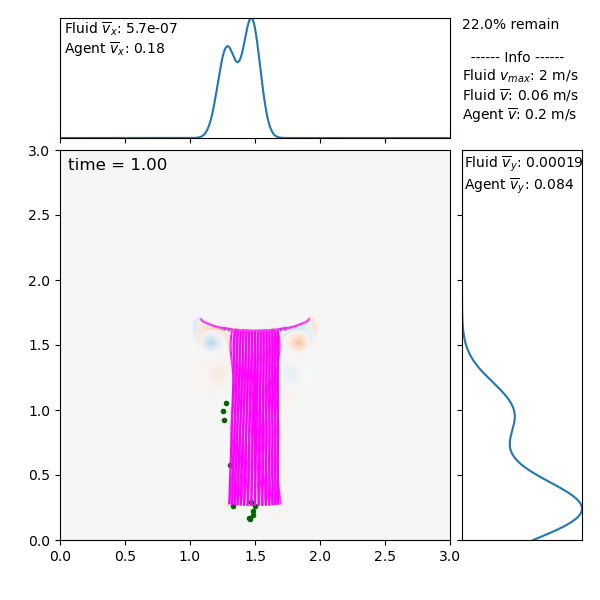
\includegraphics[width=\linewidth,height=0.43\textheight,keepaspectratio]{repo-moving-boundary-sticky.png}
\source{Sticky agents and a moving IB2d boundary; Planktos documentation image \texttt{docs/\_static/ib2d\_mvbnd\_sticky.png} (commit \texttt{a1c2128}, GPLv3).}
\begin{alertblock}{Geometry restriction}
{\footnotesize Avoid immersed structures that intersect periodic box boundaries; that interaction is not implemented in the current API.}
\end{alertblock}
{\scriptsize\hi{One more case:} a hit followed in the same step by a periodic or \texttt{noflux} box edge is lost from \texttt{ib\_collision\_idx}: the re-check at the edge resets it (to \(-1\) if nothing more is hit).\par}
\end{column}
\end{columns}
\end{frame}

% ----- 29. Stateful capture -----
\begin{frame}[fragile]{Make ``captured'' a persistent biological state}
\label{fr:capture}
\small
\begin{columns}[T,onlytextwidth]
\begin{column}{0.58\textwidth}
\begin{lstlisting}[basicstyle=\densecode]
import numpy as np
import planktos
from planktos import motion

class CaptureSwarm(planktos.Swarm):
    def apply_agent_model(self, dt):
        proposed = motion.Euler_brownian_motion(self, dt)
        held = self.get_prop("captured")[:, None]
        return np.ma.where(held, self.positions, proposed)

    def after_move(self, dt):
        hit = self.ib_collision_idx >= 0
        self.props.loc[hit, "captured"] = True
        self.props.loc[hit, "color"] = "gold"

s = CaptureSwarm(
    envir=env, ib_condition="sticky",
    store_prop_history=True)
s.props["captured"] = np.zeros(s.N, dtype=bool)
s.props["color"] = np.full(s.N, s.shared_props["color"])
\end{lstlisting}
\end{column}
\begin{column}{0.38\textwidth}
\centering

\includegraphics[width=\linewidth,height=0.27\textheight,keepaspectratio]{jeb2023-fig6a-polyp-array.png}
\source{Cylinder and polyp geometry: Hamlet et al. (2023), Fig.~6A, CC BY 4.0.}
\begin{block}{Why both hooks?}
\texttt{after\_move} records new contacts after collision correction. \texttt{apply\_agent\_model} prevents previously captured agents from leaving on later steps.
\end{block}
\end{column}
\end{columns}
\source{Pattern adapted from \texttt{examples/ex\_sticky\_seafan\_3d.py}.}
\end{frame}

% ----- 30. IB2d import -----
\begin{frame}[fragile]{Import an \NoCaseChange{IB2d} velocity field and 2D mesh}
\small
\begin{columns}[T,onlytextwidth]
\begin{column}{0.59\textwidth}
\begin{lstlisting}
env = planktos.Environment()

# From the repository root, first follow
# examples/ib2d_data/README.txt to download the data.
env.read_IB2d_fluid_data(
    "examples/ib2d_data",
    dt=5.0e-5, print_dump=1000)

env.read_IB2d_mesh_data(
    "examples/ib2d_data/channel.vertex",
    method="proximity")

env.plot_envir()
s = planktos.Swarm(
    envir=env, init=(0.1*env.L[0], 0.5*env.L[1]),
    seed=1)
\end{lstlisting}
\end{column}
\begin{column}{0.37\textwidth}
\begin{block}{Time mapping}
\footnotesize
Successive printed flow snapshots are separated by
\[
  \Delta t_{\mathrm{data}}
  =\texttt{dt}\times\texttt{print\_dump}=0.05.
\]
\end{block}
\begin{block}{Mesh association}
\footnotesize
\texttt{proximity} connects nearby vertices. It can infer resolution from loaded flow or accept \texttt{res=} explicitly.
\end{block}
{\footnotesize\warn{Inspect connectivity.} Crossing segments without a shared vertex can create collision leaks. Always call \texttt{plot\_envir()}.}
\end{column}
\end{columns}
\source{Adapted from \texttt{examples/ex\_ib2d\_ibmesh.py}; the external dataset is linked from \texttt{examples/ib2d\_data/README.txt}.}
\end{frame}

% ----- 30b. This series' IB2d output (1/2) -----
\begin{frame}[fragile]{This series' IB2d output (1/2): reading chapter 4f's starfish run}
\label{fr:starfish}
\small
\begin{columns}[T,onlytextwidth]
\begin{column}{0.56\textwidth}
\begin{lstlisting}
env = planktos.Environment(x_bndry="periodic",
    y_bndry="noflux", rho=1000, mu=0.1, units="m")
env.read_IB2d_fluid_data("Starfish_Channel/viz_IB2d",
    dt=5e-5, print_dump=400, d_start=1)
print(env.L, env.flow_times[[0, -1]],
      env.fluid_domain_LLC)
# [0.9999974399999999, 0.24999936] [0.   0.38] (0.0, 0.0)
\end{lstlisting}
\end{column}
\begin{column}{0.40\textwidth}
\footnotesize
\begin{alertblock}{Start at dump 1}
pyIB2d writes dump 0's velocity transposed: \texttt{u.0000.vtk} and \texttt{uX.0000.vtk} say \texttt{DIMENSIONS 128 512 1}, every later dump \texttt{512 128 1} (\texttt{IBM\_Driver.py} passes \texttt{U, V} there and \texttt{U.T, V.T} afterwards; \texttt{Omega} and \texttt{uMag} are right). From dump 0 the reader stops: ``all the input array dimensions \dots\ must match''.
\end{alertblock}
\end{column}
\end{columns}
\footnotesize
\begin{itemize}\itemsep1pt
  \item The fluid is at rest in dump 0, so only the run's first 0.02 s (the pulse starting from rest) is lost; Planktos's clock starts at the first dump it reads: Planktos's \(t\) is the run's \(t-0.02\) s. IB2d's issue \#12 reports the same transposed dump 0 for the MATLAB version.
  \item \texttt{L} is \(0.99999744\), not 1: IB2d writes the grid spacing with six digits (\texttt{SPACING 0.00195312}).
  \item \texttt{rho} and \texttt{mu} go to the constructor (slide~\ref{fr:inertial}). IB2d is periodic, and the reader always adds the periodic end points (its docstring's \texttt{auto\_regrid} is not a parameter).
\end{itemize}
\source{\texttt{examples/Planktos/starfish\_env.py}; \url{https://github.com/nickabattista/IB2d/issues/12} (open, 17 October 2026).}
\end{frame}

% ----- 30c. This series' IB2d output (2/2) -----
\begin{frame}[fragile]{This series' IB2d output (2/2): joining the starfish's outline}
\label{fr:starfishmesh}
\begin{lstlisting}
# starfish_only.vertex: the 405 starfish points of starfish_channel.vertex, without the walls
env.read_IB2d_mesh_data("starfish_only.vertex", method="adjacent",
                        add_idx_list=[(404, 0)])     # 0-based: last point to first
\end{lstlisting}
\scriptsize
\begin{tabular}{@{}p{0.46\textwidth}p{0.48\textwidth}@{}}
\toprule
call & what it gave (405 points, 0.503--0.566 grid cells apart) \\
\midrule
\texttt{method="adjacent", periodic=True} & 404 segments: still open (\texttt{periodic} is read only for moving meshes) \\
\texttt{add\_idx\_list=[(405, 1)]} (1-based, as the docstring says) & \texttt{IndexError}: the indices are used from 0 \\
\texttt{add\_idx\_list=[(404, 0)]} & 405 segments, closed \\
\texttt{method="proximity"} (joins points closer than \(0.501\,\Delta x\)) & 13 segments; 381 points joined to nothing \\
\texttt{method="proximity", res\_factor=0.6} & 442 segments: closed, plus 37 chords across \\
\bottomrule
\end{tabular}
\footnotesize
\begin{itemize}\itemsep1pt
  \item The channel walls (\(y=0.01\) and \(0.24\)) run across the box and cross its periodic \(x\) boundary, which Planktos does not handle (slide~\ref{fr:collide}): load the starfish alone, and let \texttt{noflux} box edges stand in for the walls.
  \item Count the segments (\texttt{len(env.ibmesh)}) as well as looking at \texttt{plot\_envir()}: a 0.57-cell gap (1.1 mm) does not show.
\end{itemize}
\source{\texttt{examples/Planktos/starfish\_env.py} (the \texttt{adjacent} call) and its \texttt{README.md} (each option tried on the same 405 points); \texttt{Environment.read\_IB2d\_mesh\_data} (\texttt{planktos/\_environment.py}, 1.0.3).}
\end{frame}

% ----- 30d. The capture pattern on the starfish -----
\begin{frame}{The capture pattern on this series' starfish}
\label{fr:capstar}
\centering
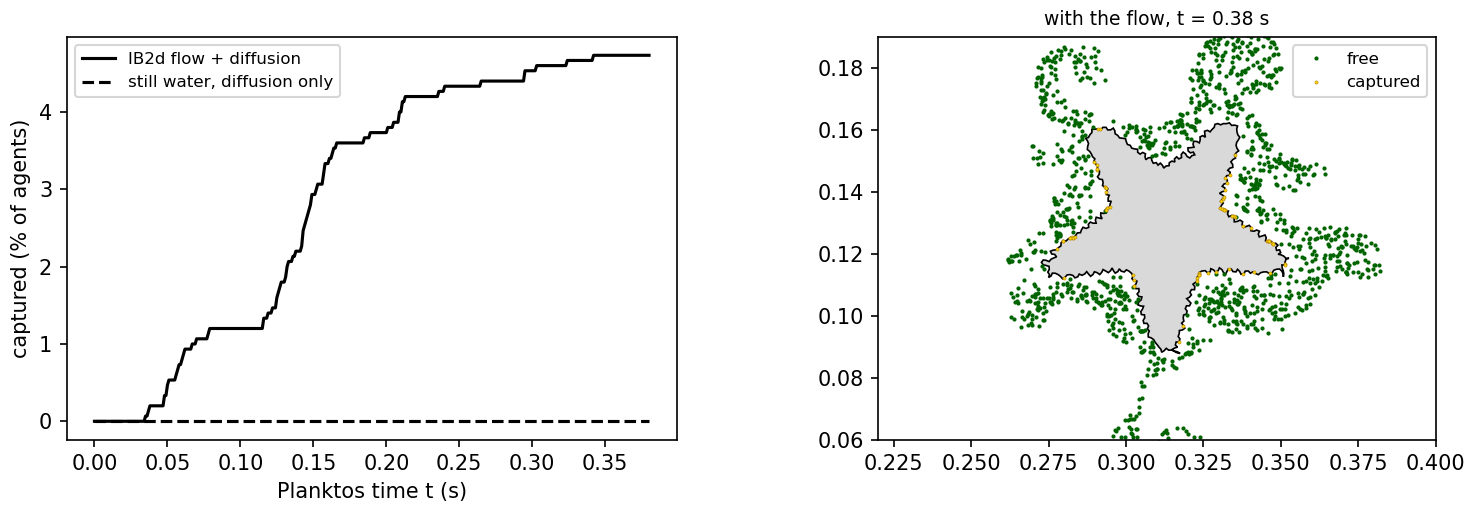
\includegraphics[width=0.84\textwidth]{planktos-starfish-capture.png}
\footnotesize
\begin{itemize}\itemsep1pt
  \item The \texttt{CaptureSwarm} of slide~\ref{fr:capture} (without its colour column), \texttt{ib\_condition="sticky"}, the starfish of the previous slide: 1500 agents start within 1.5 cm of the outline (no closer than one grid cell), \texttt{cov} \(=2\times10^{-6}\) (\(D=10^{-6}\) m\(^2\)/s), \(\Delta t = 1\) ms.
  \item With the flow 4.7\,\% are held by \(t = 0.38\) s; in still water (the same environment with \texttt{flow} set to zeros, the same seed) none. Diffusion alone moves an agent about 0.9 mm in 0.38 s (\(\sqrt{2Dt}\) in each direction): the flow brings them to the surface.
\end{itemize}
\source{\texttt{examples/Planktos/starfish\_capture.py} (Planktos 1.0.3, 90 s for both runs).}
\end{frame}

% ----- 31. Other imports -----
\begin{frame}[fragile]{Import matrix: CFD fields and 3D geometry}
\scriptsize
\begin{tabular}{@{}>{\raggedright\arraybackslash}p{0.18\linewidth}>{\raggedright\arraybackslash}p{0.47\linewidth}>{\raggedright\arraybackslash}p{0.28\linewidth}@{}}
\toprule
\textbf{Source} & \textbf{Current call pattern} & \textbf{Audit item} \\
\midrule
IBAMR 3D VTK & \texttt{env.read\_IBAMR3d\_vtk\_data(path, d\_start=0, d\_finish=None, vel\_conv=None, grid\_conv=None)} & dump range; spatial and velocity conversions \\
\addlinespace
COMSOL VTU & \texttt{env.read\_comsol\_vtu\_data(file, vel\_conv=None, grid\_conv=None)} & cell-centered versus nodal grid; units \\
\addlinespace
NetCDF & \texttt{env.load\_NetCDF(file)} then \texttt{env.read\_NetCDF\_flow("u","v", time\_name="time", dim\_reorder=...)} & variable names, dimension order, component axis, calendar/time units \\
\addlinespace
STL mesh & \texttt{env.read\_stl\_mesh\_data(file, unit\_conv=None)} & mesh and flow share the same coordinate frame \\
\addlinespace
IB2d mesh & \texttt{env.read\_IB2d\_mesh\_data(file, method="adjacent"|"proximity"|"hull")} & breaks/additional edges; closed geometry \\
\bottomrule
\end{tabular}

\vspace{0.55em}
\begin{punchbox}
\centering
The loader may reset \texttt{env.L} to match the data. Read back \texttt{L}, \texttt{flow\_points}, \texttt{flow\_times}, \texttt{fluid\_domain\_LLC}, and units after every import.
\end{punchbox}
\source{Signatures audited against \texttt{planktos/\_environment.py}, v1.0.3.}
\end{frame}

% ----- 32. Mesh and unit QA -----
\begin{frame}[fragile]{Align flow, mesh, and physical units before release}
\label{fr:qa}
\begin{columns}[T,onlytextwidth]
\begin{column}{0.54\textwidth}
\begin{lstlisting}[basicstyle=\densecode]
# For appropriate cell-centered COMSOL data,
# regrid immediately after the flow import.
# Match these flags to the data's actual BCs;
# this example treats all axes as nonperiodic (the repository's
# sea-fan example passes (True, True, True) for its COMSOL data).
env.center_cell_regrid(
    periodic_dim=(False, False, False))

# Only then load the immersed geometry.
env.read_stl_mesh_data("geometry.stl")

print("domain:", env.L, env.units)
print("flow origin:", env.fluid_domain_LLC)
print("flow axes:", [p[[0, -1]] for p in env.flow_points])
print("mesh shape:", None if env.ibmesh is None
      else env.ibmesh.shape)

env.plot_envir()
env.plot_flow()
\end{lstlisting}
\end{column}
\begin{column}{0.42\textwidth}
\footnotesize
\begin{block}{One consistent conversion ledger}
Record conversions for length, velocity, time, density, viscosity, gravity, particle diameter, and mesh coordinates. Prefer converting on import with \texttt{vel\_conv}, \texttt{grid\_conv}, or \texttt{unit\_conv}.
\end{block}
\begin{alertblock}{Visual mesh audit}
Look for crossing edges, missing closure, duplicated surfaces, mesh outside the flow domain, and unintended contact with a periodic face.
\end{alertblock}
{\scriptsize\hi{Pass the flags explicitly:} in v1.0.3 the \texttt{center\_cell\_regrid} docstring states a default of \texttt{(True, True, False)}, but the signature default is \texttt{(False, False, False)}. The regrid does not shift meshes already loaded, hence ``only then''.\par}
\end{column}
\end{columns}
\end{frame}

% ----- 32b. IBAMR -> Planktos (1/2) -----
\begin{frame}[fragile]{From an IBAMR run to Planktos (1/2): the route}
\label{fr:ibamr}
\begin{lstlisting}[basicstyle=\densecode]
# 1. VisIt (chapter 33): the AMR data on a uniform grid, as legacy VTK (here IBFE/10's last dump, around the plate)
visit -nowin -cli -s resample_export.py -- viz_IB3d/dumps.visit U plate_visit \
      nx=97 ny=49 nz=49 x0=-4 x1=8 y0=-3 y1=3 z0=-3 z1=3 states=20 format=binary
# 2. the velocity made the active vector; files named IBAMR_db_000.vtk, IBAMR_db_001.vtk, ...
python vtk_for_planktos.py plate_visit plate_planktos
# 3. Planktos: one file is a steady flow; a folder of IBAMR_db_###.vtk files, a time series
env = planktos.Environment(rho=1.0, mu=0.01)
env.read_IBAMR3d_vtk_data("plate_planktos/IBAMR_db_000.vtk")
print(env.L, env.fluid_domain_LLC, env.flow_times)   # [12.0, 6.0, 6.0] (-4.0, -3.0, -3.0) None
\end{lstlisting}
\footnotesize
\begin{itemize}\itemsep1pt
  \item Step 2 because VisIt 3.5 exports the vector as a field array beside an active scalar, and Planktos's reader then stops (``AttributeError: 'NoneType' object has no attribute 'GetDataType'''). VTK 9.4 may also print ``Could not read dimensions or extents from the file'' for these binary files: the grid still comes out whole.
  \item In 2021 this needed a Python 2.7 environment with VisIt (slide~\ref{fr:then}); now VisIt's own Python 3 does step 1.
  \item Spacing 0.125, twice the finest level's (chapter 22): \(97\times49\times49\) points, 7.5 MB. The whole \(32\times16\times16\) tank at that spacing would be about 18 times as many points.
\end{itemize}
\source{\texttt{wsl/final/ch35\_plate\_export.sh} (VisIt 3.5.0, 8 s); \texttt{examples/analysis/vtk\_for\_planktos.py}; \texttt{examples/Planktos/ibamr\_plate.py}.}
\end{frame}

% ----- 32c. IBAMR -> Planktos (2/2) -----
\begin{frame}{From an IBAMR run to Planktos (2/2): agents past IBFE/10's plate}
\label{fr:plate}
\centering
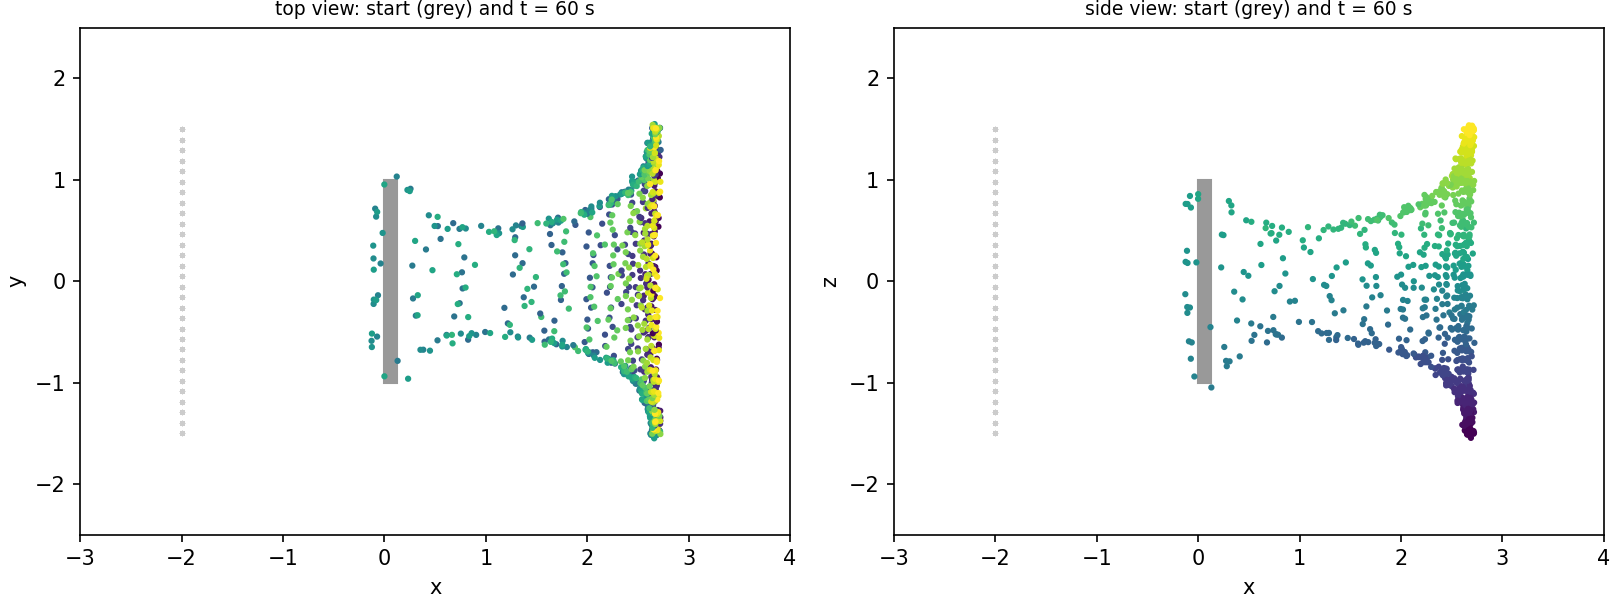
\includegraphics[width=0.67\textwidth]{planktos-ibamr-plate.png}
\footnotesize
\begin{itemize}\itemsep1pt
  \item The plate is its reference shape, a box \(0<x<0.125\), \(-1<y,z<1\), written as an STL file (12 triangles, numpy-stl) in the run's coordinates; \texttt{read\_stl\_mesh\_data} shifts it with the flow (to \(x = 4\)--\(4.125\)). By \(t = 0.5\) its flaps had bent 0.012 at their edges (chapter 22).
  \item 900 tracers, a \(30\times30\) sheet at \(x=-2\), with a little diffusion; 600 steps of 0.1 s: 86 agent-steps touched the plate (sliding). The sheet bends round the plate, the agents behind it lag in its wake, and 18 still sit against its upstream face.
  \item The last dump stands in for a steady flow; the stream was still speeding up (\(U\tanh 2t\) is 76\,\% of \(U\) at \(t=0.5\)), so a longer run would give a truer one.
\end{itemize}
\source{\texttt{examples/Planktos/ibamr\_plate.py} (Planktos 1.0.3, 40 s); IBFE/10 (chapter 22).}
\end{frame}

% ----- 33. FTLE -----
\begin{frame}[fragile]{FTLE reveals finite-time stretching of a motion model}
\label{fr:ftle}
\small
\begin{columns}[T,onlytextwidth]
\begin{column}{0.53\textwidth}
Let \(\tau=T-t_0>0\). For the flow map \(\vect\Phi_{t_0}^{T}\), the largest forward-time exponent is
\[
  \sigma_{t_0}^{\tau}(\vect x_0)
  =\frac{1}{\tau}\log\sqrt{\lambda_{\max}\!\left[(D\vect\Phi)^T D\vect\Phi\right]}.
\]
\begin{lstlisting}[basicstyle=\densecode]
env.calculate_FTLE(
    grid_dim=(512, 128),
    t0=0, T=0.1, dt=0.001)
env.plot_2D_FTLE()

# Backward from physical time 0.1 to 0.0:
# current API uses T as the forward pseudo-time endpoint.
env.calculate_FTLE(
    (512, 128), t0=0.1, T=0.2,
    dt=0.001, backward=True)
\end{lstlisting}
\vspace{-2pt}
\source{Calls adapted from \texttt{examples/ex\_produce\_ftle\_2d.py}.}
\end{column}
\begin{column}{0.44\textwidth}
\centering
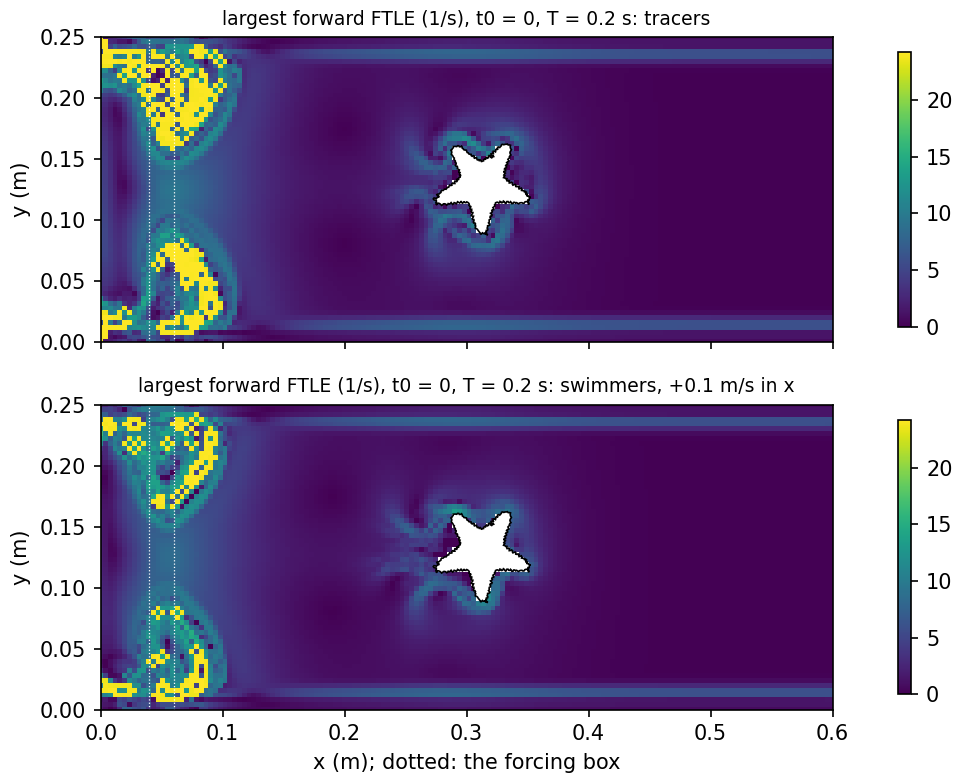
\includegraphics[width=\linewidth,height=0.27\textheight,keepaspectratio]{planktos-starfish-ftle.png}
\source{The first call on this series' starfish flow (\(256\times64\) points, \texttt{T=0.2}, \texttt{testdir="x1"}, \texttt{dt=0.002}) for tracers (top) and, with \texttt{swrm=}, for swimmers that add 0.1 m/s in \(x\) (bottom): \texttt{examples/Planktos/starfish\_ftle.py}, 140 s per map. Strickland et al.\ (2022), Fig.~5, compares FTLE fields for parasitoid wasps (not reproduced).}
\begin{alertblock}{Two API distinctions}
{\scriptsize\begin{itemize}\itemsep0pt
  \item The current call requires \texttt{T > t0}; the elapsed interval is \texttt{T-t0} (\texttt{T} is an end time, although the docstring calls it ``integration time'' and \texttt{plot\_2D\_FTLE}'s title prints it as \(\Delta t\)). With \texttt{backward=True}, physical time ends at \texttt{2*t0-T}; tracers only.
  \item \texttt{FTLE\_smallest} is a forward-map contraction exponent, not backward-time FTLE.
\end{itemize}}
\end{alertblock}
\end{column}
\end{columns}
\end{frame}

% ----- 34. FTLE validity -----
\begin{frame}{When an agent-based FTLE field is meaningful}
\footnotesize
\begin{columns}[T,onlytextwidth]
\begin{column}{0.56\textwidth}
The \texttt{swrm=} route is appropriate when the seeded agents define one reproducible finite-time map:
\begin{itemize}\itemsep4pt
  \item the motion rule is deterministic;
  \item agents use the same rule and parameter set;
  \item each trajectory acts independently of the other seeded agents;
  \item the map is resolved well enough in time and on the initial-condition grid.
\end{itemize}
\begin{alertblock}{Not an ordinary FTLE map}
Stochastic realizations or social rules that depend on the seeded population do not define a single deterministic particle map. Use ensemble dispersion, encounter, or density diagnostics instead.
\source{Qualification follows Strickland et al. (2022), Sections 2.1 and 4.2.}
\end{alertblock}
\end{column}
\begin{column}{0.40\textwidth}
\centering
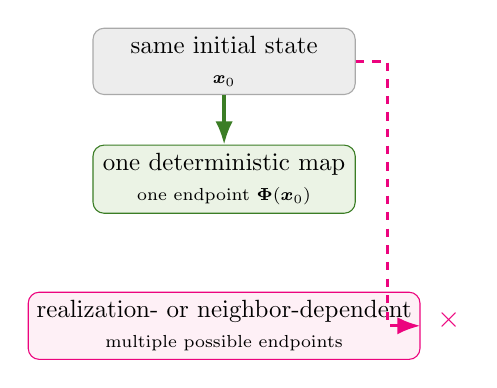
\begin{tikzpicture}[>=Latex,node distance=7mm,scale=0.90,transform shape]
  \node[draw=DarkGray,rounded corners,fill=LightGray!40,align=center,minimum width=3.7cm,minimum height=0.9cm] (x0) {same initial state\\\scriptsize \(\vect x_0\)};
  \node[draw=plankgreen,rounded corners,fill=OliveGreen!8,align=center,minimum width=3.7cm,minimum height=0.9cm,below=of x0] (one) {one deterministic map\\\scriptsize one endpoint \(\vect\Phi(\vect x_0)\)};
  \draw[->,very thick,plankgreen] (x0)--(one);
  \node[draw=RubineRed,rounded corners,fill=RubineRed!6,align=center,minimum width=3.7cm,minimum height=0.9cm,below=11mm of one] (many) {realization- or neighbor-dependent\\\scriptsize multiple possible endpoints};
  \draw[->,very thick,RubineRed,dashed] (x0.east) -- ++(0.45,0) |- (many.east);
  \node[RubineRed,font=\bfseries\large] at ([xshift=4mm,yshift=-4mm]many.north east) {\(\times\)};
\end{tikzpicture}
\vspace{0.4em}
\begin{punchbox}
\centering
FTLE is a property of the chosen finite-time map, not of ``complex-looking'' trajectories in general.
\end{punchbox}
\source{Schematic: instructor's course notes.}
\end{column}
\end{columns}
\end{frame}

% ----- 35. Capstone setup -----
\begin{frame}[fragile]{Capstone: Vicsek agents around an immersed cylinder}
\small
\begin{columns}[T,onlytextwidth]
\begin{column}{0.56\textwidth}
\begin{lstlisting}
import numpy as np
import planktos

env = planktos.Environment(
    Lx=1, Ly=0.25,
    x_bndry="periodic",
    y_bndry="periodic")
env.read_IB2d_mesh_data(
    "examples/vicsek_mesh/channel.vertex",
    method="proximity", res=0.001953125)

rng = np.random.default_rng(2026)
N = 500
IC = np.empty((N, 2))
IC[:, 0] = rng.uniform(0.075, 0.125, N)
IC[:, 1] = rng.uniform(0.050, 0.200, N)
\end{lstlisting}
\end{column}
\begin{column}{0.40\textwidth}
\centering
\begin{block}{Null versus flow experiment}
The repository example runs without the large external flow dataset. Load matching IB2d flow to ask how alignment survives an unsteady wake: slide~\ref{fr:vicsekstar} does it with this series' starfish flow.
\end{block}
{\scriptsize Strickland et al.\ (2022), Fig.~9, motivates the capstone with a 3D Vicsek result in cylinder flow (not reproduced: the article is not openly licensed).\par}
\end{column}
\end{columns}
\source{Setup: current \texttt{examples/ex\_vicsek\_model\_2d.py}; separate NumPy seed added.}
\end{frame}

% ----- 36. Capstone model -----
\begin{frame}[fragile]{Capstone: implement alignment with periodic distances}
\small
\begin{columns}[T,onlytextwidth]
\begin{column}{0.68\textwidth}
\begin{lstlisting}[basicstyle=\densecode]
class Vicsek(planktos.Swarm):
    def __init__(self, *args, **kwargs):
        super().__init__(*args, **kwargs)
        self.shared_props.update(v=0.02, nu=0.5, r=0.1)
        angle = self.get_prop("nu") \
              * (self.rndState.random(self.N)-0.5)
        self.velocities += self.get_prop("v") \
              * np.column_stack((np.cos(angle), np.sin(angle)))

    def apply_agent_model(self, dt):
        theta = np.empty(self.N)
        L = np.asarray(self.envir.L)
        for i, origin in enumerate(self.positions):
            delta = (self.positions-origin + L/2) % L - L/2
            near = np.linalg.norm(delta, axis=1) < self.get_prop("r")
            theta[i] = np.arctan2(
                self.velocities[near, 1].mean(),
                self.velocities[near, 0].mean())
        theta += self.get_prop("nu")*(self.rndState.random(self.N)-0.5)
        active = self.get_prop("v")*np.column_stack((np.cos(theta), np.sin(theta)))
        return self.positions + (active + self.get_fluid_drift())*dt
\end{lstlisting}
\end{column}
\begin{column}{0.30\textwidth}
\footnotesize
\begin{block}{Three model ingredients}
\begin{enumerate}\itemsep1pt
  \item average neighbor velocity vectors within radius \texttt{r};
  \item add angular noise of width \texttt{nu};
  \item add self-propulsion speed \texttt{v} and local fluid drift.
\end{enumerate}
\end{block}
\begin{alertblock}{Periodic metric}
{\scriptsize The minimum-image displacement is essential: agents near opposite faces can still be neighbors. Note that the minimum-image wrap assumes periodic boundaries in both axes.}
\end{alertblock}
\end{column}
\end{columns}
\source{Condensed from the current repository Vicsek example (\texttt{examples/ex\_vicsek\_model\_2d.py}); parameter names and hook are unchanged. Model: Vicsek et al.\ (1995).}
\end{frame}

% ----- 36b. Capstone model: reading the rule -----
\begin{frame}{Capstone: what the alignment rule actually averages}
\small
In the notation of Vicsek et al.\ (1995), each agent \(i\) updates its heading as
\[
  \theta_i^{n+1}=\arg\!\Big(\sum_{j:\,|\vect x_j-\vect x_i|<r}\vect v_j^{\,n}\Big)+\xi_i^n,
  \qquad \xi_i^n\sim\mathcal U\!\left[-\tfrac{\eta}{2},\tfrac{\eta}{2}\right],
\]
then moves with \(\vect x_i^{n+1}=\vect x_i^n+\big[v\,(\cos\theta_i^{n+1},\sin\theta_i^{n+1})+\vect u(\vect x_i^n,t^n)\big]\Delta t\). Here \(\eta\) is \texttt{nu}, \(v\) is \texttt{v}, and \(r\) is \texttt{r}.
\begin{itemize}\itemsep1.5pt
  \item Because \texttt{move} sets \texttt{velocities} from each step's displacement over \texttt{dt} (the proposed one, or the slide along a mesh), the neighbor average uses ground-frame velocities (swimming plus fluid drift), not swimming headings alone. In a strong flow the fluid can dominate the ``consensus''.
  \item An agent always counts itself as a neighbor (distance \(0<r\)), so the average is never empty.
  \item The condensed listing wraps both axes unconditionally; the repository version wraps only the axes whose \texttt{envir.bndry} is \texttt{periodic}, so use that form in a channel with walls.
  \item The noise is drawn once per step, so the statistics depend on \(\Delta t\); this is why the capstone asks for at least two smaller \(\Delta t\).
  \item A standard summary is the polarization \(\varphi=\big|\sum_i \vect s_i\big|/(Nv)\in[0,1]\), with \(\vect s_i\) the self-propulsion velocity; \(\varphi\approx1\) is an aligned flock.
\end{itemize}
\source{Vicsek et al.\ (1995), Eqs.~(1)--(2) and their order parameter; Planktos example \texttt{ex\_vicsek\_model\_2d.py}, commit \texttt{a1c2128}.}
\end{frame}

% ----- 36c. The capstone's rule around the starfish -----
\begin{frame}{Capstone: the rule around this series' starfish}
\label{fr:vicsekstar}
\centering
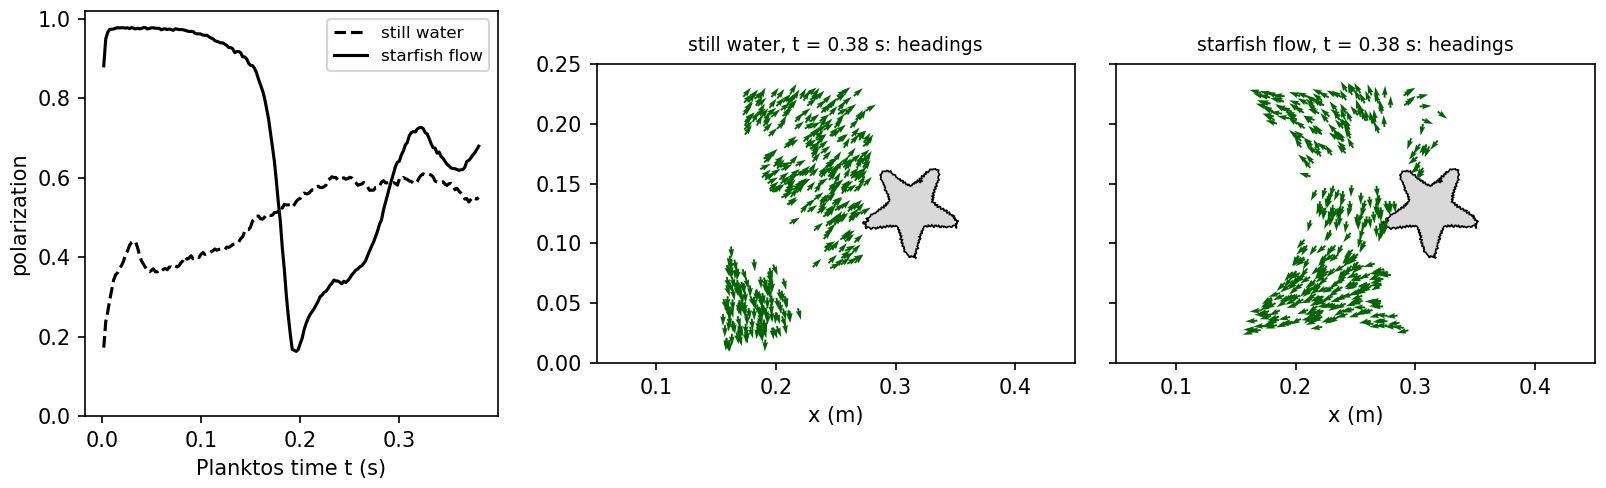
\includegraphics[width=0.86\textwidth]{planktos-starfish-vicsek.png}
\footnotesize
\begin{itemize}\itemsep1pt
  \item The capstone's rule with all pairs at once (no loop), the minimum image on the periodic \(x\) axis only, and random starting headings: 400 agents released upstream of chapter 4f's starfish, \(v=0.1\) m/s, \(r=2\) cm, \texttt{nu} \(=0.5\), \(\Delta t = 2\) ms, for the run's 0.38 s.
  \item Still water: the polarization grows from 0.17 to about 0.6 (0.55 at the end), and the swarm splits into two groups. The flow: 0.88 after the first step and 0.98 by \(t=0.02\) s, because the neighbours' mean velocity is the stream's (previous slide); briefly below 0.2 (0.16 at \(t=0.196\) s) as the stream near the agents dies away (its mean \(u\) from 0.31 m/s at \(t=0.08\) s to 0 at \(t=0.18\) s); 0.68 at the end.
\end{itemize}
\source{\texttt{examples/Planktos/starfish\_vicsek.py} (Planktos 1.0.3, 25 s for both runs).}
\end{frame}

% ----- 37. Run and validate -----
\begin{frame}[fragile]{Run the capstone, then make the result reproducible}
\footnotesize
\begin{columns}[T,onlytextwidth]
\begin{column}{0.55\textwidth}
\begin{lstlisting}
s = Vicsek(
    swarm_size=N, envir=env, init=IC, seed=2026)

collision_events = 0
for _ in range(72):       # 18 s at dt=0.25 s
    s.move(0.25, silent=True)
    collision_events += np.count_nonzero(
        s.ib_collision_idx >= 0)

print("agent-step collisions:", collision_events)

s.plot_all(
    movie_filename="vicsek_null.mp4",
    fps=4, fluid="vort")
\end{lstlisting}
\begin{block}{Capstone comparisons}
{\footnotesize Repeat with a passive swarm, multiple \texttt{nu}/\texttt{r} values, and at least two smaller \(dt\). Compare polarization, retention, agent-step collisions, and downstream spread.}
\end{block}
\end{column}
\begin{column}{0.41\textwidth}
\begin{block}{Save with every result}
{\scriptsize\begin{itemize}\itemsep0pt
  \item Planktos version/commit and Python/package environment;
  \item flow and mesh provenance plus checksums;
  \item both random seeds and all model parameters;
  \item time step, duration, collision mode, and active-agent count;
  \item code, raw histories, and plotting settings.
\end{itemize}}
\end{block}
\begin{alertblock}{Failure-state diagnostic}
{\scriptsize If a collision step fails, current Planktos marks \texttt{env.time=None}. Inspect the partial state; then restore consistently from histories or restart from a checkpoint.}
\end{alertblock}
\end{column}
\end{columns}
\end{frame}

% ----- 37b. This series' examples -----
\begin{frame}{This series' Planktos examples}
\label{fr:ourexamples}
\scriptsize
\begin{tabular}{@{}p{0.27\textwidth}p{0.55\textwidth}p{0.11\textwidth}@{}}
\toprule
\texttt{examples/Planktos/} & what it does & slides \\
\midrule
\texttt{brinkman\_first.py} & most of this chapter's first-run fragments, in order: Brinkman flow, a swarm, 24 s, plots, \texttt{save\_data}, CSV, VTK (a movie if FFmpeg is found; not run here, without FFmpeg); no input data & \ref{fr:plot} \\
\texttt{starfish\_env.py} & \texttt{load(run)}: chapter 4f's starfish run as an \texttt{Environment}, the starfish as a closed mesh & \ref{fr:starfish}, \ref{fr:starfishmesh} \\
\texttt{starfish\_kde.py} & agents upstream of the starfish; vorticity and KDEs & \ref{fr:kde} \\
\texttt{starfish\_capture.py} & the capture pattern, with the flow and in still water & \ref{fr:capstar} \\
\texttt{starfish\_ftle.py} & FTLE maps for tracers and for swimmers & \ref{fr:ftle} \\
\texttt{starfish\_vicsek.py} & the capstone's rule in still water and in the flow & \ref{fr:vicsekstar} \\
\texttt{ibamr\_plate.py} & IBFE/10's flow tank through VisIt; a sheet of agents past the plate & \ref{fr:ibamr}, \ref{fr:plate} \\
\bottomrule
\end{tabular}

\vspace{1mm}
\footnotesize Run on Planktos 1.0.3 (git \texttt{a1c2128}) with Python 3.12 (Anaconda, Windows) on a desktop PC; the folder's \texttt{README.md} gives each script's time and result. The starfish run is chapter 4f's example (pyIB2d), IBFE/10 chapter 22's.
\source{\texttt{examples/Planktos/README.md}.}
\end{frame}

% ----- 37c. Known issues -----
\begin{frame}{Known issues in 1.0.3, and what this chapter does about them (1/2)}
\label{fr:issues}
\scriptsize
\begin{tabular}{@{}p{0.55\textwidth}p{0.39\textwidth}@{}}
\toprule
issue (October 2026) & what to do \\
\midrule
the \texttt{nu} and \texttt{rho} setters compute \(\mu=\nu/\rho\) (slide~\ref{fr:inertial}) & give \texttt{rho} and \texttt{mu} (or \texttt{nu}) to the constructor \\
\texttt{center\_cell\_regrid}: docstring default \texttt{(True, True, False)}, signature \texttt{(False, False, False)} (slide~\ref{fr:qa}) & pass \texttt{periodic\_dim} explicitly \\
\texttt{read\_IB2d\_mesh\_data} on a \texttt{.vertex} file with \texttt{'adjacent'}: \texttt{periodic=True} ignored; \texttt{add\_idx\_list} used from 0, documented from 1 (slide~\ref{fr:starfishmesh}) & close an outline with \texttt{add\_idx\_list=[(n-1, 0)]}; count the segments \\
\texttt{read\_IB2d\_fluid\_data}: the docstring lists an \texttt{auto\_regrid} parameter the signature does not have & nothing: the periodic end points are always added \\
\texttt{calculate\_FTLE}: the docstring speaks of an \texttt{ode} argument (it is \texttt{ode\_gen}) and says ``Default is 1'' for \texttt{T}, whose default is 0.1; \texttt{T} is an end time (slide~\ref{fr:ftle}) & trust the signature: \texttt{inspect.signature(env.calculate\_FTLE)} \\
\bottomrule
\end{tabular}

\vspace{1mm}
\footnotesize The pyIB2d item, four more traps of 1.0.3 met while running this chapter's fragments, and the search of Planktos's issues are on the next slide.
\source{\texttt{planktos/\_environment.py} (1.0.3); \texttt{examples/Planktos}.}
\end{frame}

% ----- 37d. Known issues (2/2) -----
\begin{frame}{Known issues in 1.0.3, and what this chapter does about them (2/2)}
\label{fr:issues2}
\scriptsize
\begin{tabular}{@{}p{0.55\textwidth}p{0.39\textwidth}@{}}
\toprule
issue (October 2026) & what to do \\
\midrule
pyIB2d writes dump 0's velocity transposed (IB2d issue \#12; slide~\ref{fr:starfish}) & read from dump 1 \\
\texttt{Swarm.plot\_all(fluid="vort")} on a static flow, such as the Brinkman layer (slide~\ref{fr:animate}), stops with ``ValueError: not enough values to unpack (expected 2, got 1)'' (\texttt{\_swarm.py}, line 2548), with or without a movie file & \texttt{fluid="quiver"}, or none, on a static flow; \texttt{"vort"} works on a time-dependent one \\
\texttt{init="grid"} with \texttt{testdir} and no immersed mesh stops with ``AttributeError: 'NoneType' object has no attribute 'reshape''' (slide~\ref{fr:init}) & give \texttt{testdir} only when a mesh is loaded \\
a \code{'D'} property is read only when there is no \code{'cov'}, and every Swarm starts with \code{cov} = the identity unless given one (slide~\ref{fr:sde}) & set \code{'cov'} to \(2D\), or delete \code{'cov'} before setting \code{'D'} \\
\texttt{set\_brinkman\_flow}: the docstring calls \texttt{alpha=0} free flow; the call divides by \(\alpha^2\) and stops with ``ZeroDivisionError: float division by zero'' (slide~\ref{fr:brinkman}) & a small \texttt{alpha} instead (\(10^{-6}\) gives the free-flow profile) \\
\bottomrule
\end{tabular}

\vspace{1mm}
\footnotesize Searching Planktos's issues on 17 October 2026 (\texttt{add\_idx\_list}, \texttt{periodic}, \texttt{regrid}, \texttt{setter}, \texttt{viscosity}, \texttt{docstring}, \texttt{vort}, \texttt{plot\_all}, \texttt{testdir}, \texttt{diffusion}, \texttt{brinkman}) found none of the Planktos items on these two slides; related open ones are \#75 (the 3D \texttt{.vertex} reader, chapter 34), \#33 (moving the SDE solver to Milstein) and \#74 (both fluid backdrops at once in \texttt{plot} and \texttt{plot\_all}).
\source{\texttt{planktos/\_environment.py}, \texttt{\_swarm.py} and \texttt{motion.py} (1.0.3); \texttt{examples/Planktos}; \url{https://github.com/mountaindust/Planktos/issues}.}
\end{frame}

% ----- 38. Resources -----
\begin{frame}{Resources and source trail}
\begin{columns}[T,onlytextwidth]
\begin{column}{0.55\textwidth}
\begin{block}{Start with the current software}
\small
\begin{itemize}\itemsep1pt
  \item \href{https://github.com/mountaindust/Planktos}{Planktos repository and README};
  \item repository \texttt{docs/} and runnable \texttt{examples/};
  \item \texttt{examples/ib2d\_data/README.txt} for the external IB2d dataset;
  \item this tutorial was audited against v1.0.3, commit \texttt{a1c2128} (2026-08-19);
  \item this series' \texttt{examples/Planktos} (its README: what each script gave);
  \item the lab's 2021 deck, ``Getting started with Planktos'' (install, tests, examples of 2021).
\end{itemize}
\end{block}
\begin{punchbox}
\centering\small
Record the exact software commit with every scientific result: current interfaces can differ from those shown in the 2022 paper.
\end{punchbox}
\end{column}
\begin{column}{0.41\textwidth}
\begin{block}{Primary scientific sources}
\small
\href{https://doi.org/10.1007/s11538-022-01027-1}{Strickland et al. (2022), \emph{Bulletin of Mathematical Biology} 84:72}\\[8pt]
Software architecture, agent models, collision handling, visualization, FTLE, and examples.\\[10pt]
\href{https://doi.org/10.1242/jeb.244520}{Hamlet et al. (2023), \emph{Journal of Experimental Biology} 226, jeb244520}\\[8pt]
Gorgonian multiscale flow and capture application; article and reproduced figures are CC BY 4.0.
\end{block}
\end{column}
\end{columns}
\end{frame}

% ----- 39. References -----
\begin{frame}{References}
\footnotesize
\begin{itemize}\itemsep3pt
  \item W. C. Strickland, N. A. Battista, C. L. Hamlet, and L. A. Miller, ``Planktos: an agent-based modeling framework for small organism movement and dispersal in a fluid environment with immersed structures,'' \emph{Bull. Math. Biol.} 84 (2022), 72, \href{https://doi.org/10.1007/s11538-022-01027-1}{doi:10.1007/s11538-022-01027-1}. Its Figs.~4, 5 and 9 are described, not reproduced (the article is not openly licensed): the pictures are this series' runs. FTLE qualifications from Sections 2.1 and 4.2.
  \item C. L. Hamlet, W. C. Strickland, N. Battista, and L. A. Miller, ``Multiscale flow between the branches and polyps of gorgonians,'' \emph{J. Exp. Biol.} 226(5) (2023), jeb244520, \href{https://doi.org/10.1242/jeb.244520}{doi:10.1242/jeb.244520}. CC BY 4.0; Figs.~1 and 6A reproduced.
  \item W. C. Strickland \emph{et al.}, \emph{Planktos} agent-based modeling framework, v1.0.3, commit \texttt{a1c2128} (2026-08-19), GPLv3, \url{https://github.com/mountaindust/Planktos}; documentation \url{https://planktos.readthedocs.io}. Source of every code pattern (\texttt{README.md}, \texttt{setup.cfg}, \texttt{examples/}, docstrings) and of the \texttt{docs/\_static} images.
  \item S. Kupfner Johnson and P. Hallock, ``A review of symbiotic gorgonian research in the western Atlantic and Caribbean with recommendations for future work,'' \emph{Coral Reefs} 39 (2020), 239--258, \href{https://doi.org/10.1007/s00338-020-01891-0}{doi:10.1007/s00338-020-01891-0}. Adapted in Hamlet et al.\ (2023), Fig.~1.
  \item M. R. Maxey and J. J. Riley, ``Equation of motion for a small rigid sphere in a nonuniform flow,'' \emph{Phys. Fluids} 26 (1983), 883--889, \href{https://doi.org/10.1063/1.864230}{doi:10.1063/1.864230}.
  \item G. Haller and T. Sapsis, ``Where do inertial particles go in fluid flows?'' \emph{Physica D} 237 (2008), 573--583, \href{https://doi.org/10.1016/j.physd.2007.09.027}{doi:10.1016/j.physd.2007.09.027}. Linearized form used by \texttt{inertial\_particles}.
\end{itemize}
\end{frame}

% ----- 40. References (continued) -----
\begin{frame}{References (continued)}
\footnotesize
\begin{itemize}\itemsep3pt
  \item T. Vicsek, A. Czir\'ok, E. Ben-Jacob, I. Cohen, and O. Shochet, ``Novel type of phase transition in a system of self-driven particles,'' \emph{Phys. Rev. Lett.} 75 (1995), 1226--1229, \href{https://doi.org/10.1103/PhysRevLett.75.1226}{doi:10.1103/PhysRevLett.75.1226}.
  \item S. C. Shadden, F. Lekien, and J. E. Marsden, ``Definition and properties of Lagrangian coherent structures from finite-time Lyapunov exponents in two-dimensional aperiodic flows,'' \emph{Physica D} 212 (2005), 271--304, \href{https://doi.org/10.1016/j.physd.2005.10.007}{doi:10.1016/j.physd.2005.10.007}.
  \item G. Haller, ``Lagrangian coherent structures,'' \emph{Annu. Rev. Fluid Mech.} 47 (2015), 137--162, \href{https://doi.org/10.1146/annurev-fluid-010313-141322}{doi:10.1146/annurev-fluid-010313-141322}.
  \item P. E. Kloeden and E. Platen, \emph{Numerical Solution of Stochastic Differential Equations}. Springer, 1992, \href{https://doi.org/10.1007/978-3-662-12616-5}{doi:10.1007/978-3-662-12616-5}. Euler--Maruyama (\S10.2) and Milstein (\S10.3) schemes.
  \item J. R. Dormand and P. J. Prince, ``A family of embedded Runge--Kutta formulae,'' \emph{J. Comput. Appl. Math.} 6 (1980), 19--26, \href{https://doi.org/10.1016/0771-050X(80)90013-3}{doi:10.1016/0771-050X(80)90013-3}. The RK45 pair behind \texttt{motion.RK45}.
  \item H. C. Brinkman, ``A calculation of the viscous force exerted by a flowing fluid on a dense swarm of particles,'' \emph{Appl. Sci. Res.} A1 (1949), 27--34, \href{https://doi.org/10.1007/BF02120313}{doi:10.1007/BF02120313}.
\end{itemize}
\end{frame}

% ----- 41. References (continued) -----
\begin{frame}{References (continued)}
\footnotesize
\begin{itemize}\itemsep3pt
  \item W. C. Strickland, L. A. Miller, A. Santhanakrishnan, C. Hamlet, N. A. Battista, and V. Pasour, ``Three-dimensional low Reynolds number flows near biological filtering and protective layers,'' \emph{Fluids} 2 (2017), 62, \href{https://doi.org/10.3390/fluids2040062}{doi:10.3390/fluids2040062}. Analytic Brinkman profile behind \texttt{set\_brinkman\_flow}.
  \item D. W. Scott, \emph{Multivariate Density Estimation}. Wiley, 1992, \href{https://doi.org/10.1002/9780470316849}{doi:10.1002/9780470316849}. Scott's KDE bandwidth factor (\texttt{dist="density"}).
  \item N. A. Battista, W. C. Strickland, and L. A. Miller, ``IB2d: a Python and MATLAB implementation of the immersed boundary method,'' \emph{Bioinspir. Biomim.} 12 (2017), 036003, \href{https://doi.org/10.1088/1748-3190/aa5e08}{doi:10.1088/1748-3190/aa5e08}. Source of the IB2d flow and mesh formats.
  \item FFmpeg project, \url{https://ffmpeg.org}. External movie writer used by Matplotlib for \texttt{plot\_all(movie\_filename=...)}.
\end{itemize}
\end{frame}

% ----- 41b. References (continued) -----
\begin{frame}{References (continued)}
\footnotesize
\begin{itemize}\itemsep3pt
  \item Planktos release notes v1.0.1--v1.0.3 and \texttt{README.md}, \url{https://github.com/mountaindust/Planktos} (read 17 October 2026); IB2d issue \#12, \url{https://github.com/nickabattista/IB2d/issues/12}.
  \item ``Getting started with Planktos'' (Miller lab, 2021): the install, tests and example tour merged here, and the 2021 pictures.
\end{itemize}
\begin{punchbox}
\footnotesize The workflow, object-model, Brinkman-layer, shared-clock, and FTLE-validity diagrams were drawn for these notes (TikZ). Code fragments are adapted from the Planktos repository (GPLv3) as credited on each slide; the plots are this series' runs (\texttt{examples/Planktos}), the 2021 lab deck's, and two Planktos documentation images (the title slide and slide~\ref{fr:collide}).
\end{punchbox}
\end{frame}

\end{document}
